\chapter{Materials and methods}\label{methods}
\chapterquote{"My needle is not just a weapon; it is a tool of restoration. I will stitch this broken world back together, or I will watch it unravel entirely."}{--- Hornet (Hollow Knight: Silksong)}

\newpage

With the main objectives of this work in mind, the present chapter provides a description of the computational methods employed throughout this thesis. It begins with an overview of molecular dynamics (MD) simulations, the primary simulation technique used to generate and analyze the trajectories under study. This is followed by a summary of the analytical tools used to interpret the resulting data. The chapter then turns from classical molecular-dynamics simulations to quantum-computing (QC) approaches. This thesis evaluates, as a proof of concept, whether selected peptide-folding and sequence-design problems can be formulated and explored using currently available quantum algorithms and hardware or simulators. Together, these approaches provide the framework for the conformational sampling and analysis presented in the following sections.


\section{Molecular dynamics: principles}

MD has emerged as a primary computational technique for investigating the time-dependent behavior of interacting particle systems. MD simulations numerically integrate the equations of motion for the particles in a system, tracking the dynamical evolution of molecular structures and their internal degrees of freedom over time~\cite{braun2018best}. Since its inception, MD has evolved remarkably: in their pioneering 1957 study, Alder and Wainwright simulated just over a hundred particles using a hard-sphere model to study phase transitions~\cite{alder1957phase}. Today, advances in computational power enable simulations of hundreds of thousands of atoms over microsecond timescales, requiring hundreds of millions to billions of femtosecond-scale integration steps~\cite{Acun2018,charron2025navigating}. Nevertheless, the accessible spatial and temporal scales remain fundamentally constrained by the computational cost of resolving molecular detail. Recent whole-cell simulations have extended computational modeling to cellular scales through reduced-resolution representations~\cite{THORNBURG2026}, illustrating the fundamental trade-off between molecular resolution, system size, and accessible timescales.

In this thesis, MD constitutes the main simulation methodology. The equations of motion are derived from a potential energy function defined by the chosen force field, while additional algorithms ensure that simulations maintain the desired thermodynamic conditions, such as temperature and pressure~\cite{braun2018best}. This section provides the general methodological framework and explains the physical and algorithmic principles underlying the computational approaches used throughout this work, including both conventional MD and enhanced sampling techniques. Study-specific simulation protocols are detailed in the corresponding results chapters and methods sections (see Chapters \ref{chap:results} and \ref{chap:unpublished}) of each associated article or manuscript. When previously established protocols are reused without modification, the original reference is cited explicitly; any deviations are clearly documented.

All simulations were performed using Groningen MAchine for Chemical Simulations (GROMACS)~\cite{Gromacs2015}. Its documentation is used as a reference for technical details concerning the implementation of the simulation algorithms described below.



\subsection{Foundations and integration}

Standard MD is grounded in Newton's equations of motion~\cite{leyesnewton}, which form the foundation of classical mechanics. The term \emph{classical} signifies that quantum effects, such as those governing electronic dynamics, are not treated explicitly. This pragmatic approach relies on the Born–Oppenheimer approximation, according to which nuclear and electronic motion can be treated separately. It is therefore assumed that the electron clouds adjust their dynamics instantly when the atomic positions change, and that they always remain in the ground state~\cite{born1927quantentheorie}\footnote{Nevertheless, the MD framework can be extended beyond classical empirical potentials; when chemical reactivity or explicit electronic structures are required~\cite{vennelakanti2022harder, ahmadi2018multiscale}, methodologies such as \emph{ab initio} Molecular Dynamics~\cite{car1985unified} or hybrid QM/MM~\cite{WARSHEL1976227} schemes are employed to evaluate the system at the quantum mechanical level.}

Through this approximation, the inherently complex quantum mechanical problem is effectively reduced to the time evolution of a system of \(N\) classical particles. Nevertheless, obtaining an exact analytical solution for the motion of these nuclei remains impossible, as no general closed-form analytical solution exists for a system of \(N \geq 3\) interacting particles. This challenge, known as the \emph{N-body problem}, has been extensively studied since Isaac Newton first formulated it in the 17th century in the context of celestial mechanics. The same limitation applies to molecular systems composed of \(N\) interacting particles~\cite{n-body}.

Consequently, the equations of motion must generally be solved numerically by discretizing time into finite integration steps. MD provides a computational framework for performing this numerical integration and describing the resulting time evolution of interacting-particle systems~\cite{braun2018best,biblia_2}.

In practice, MD simulations generate system trajectories by iteratively updating particle positions and momenta at successive time steps. Repetition of this procedure over a large number of iterations enables an accurate representation of the system’s dynamical behavior. The general workflow of a standard MD simulation is summarized in Figure~\ref{fig:MDFlow}.
\begin{figure}[!htbp]
    \centering
    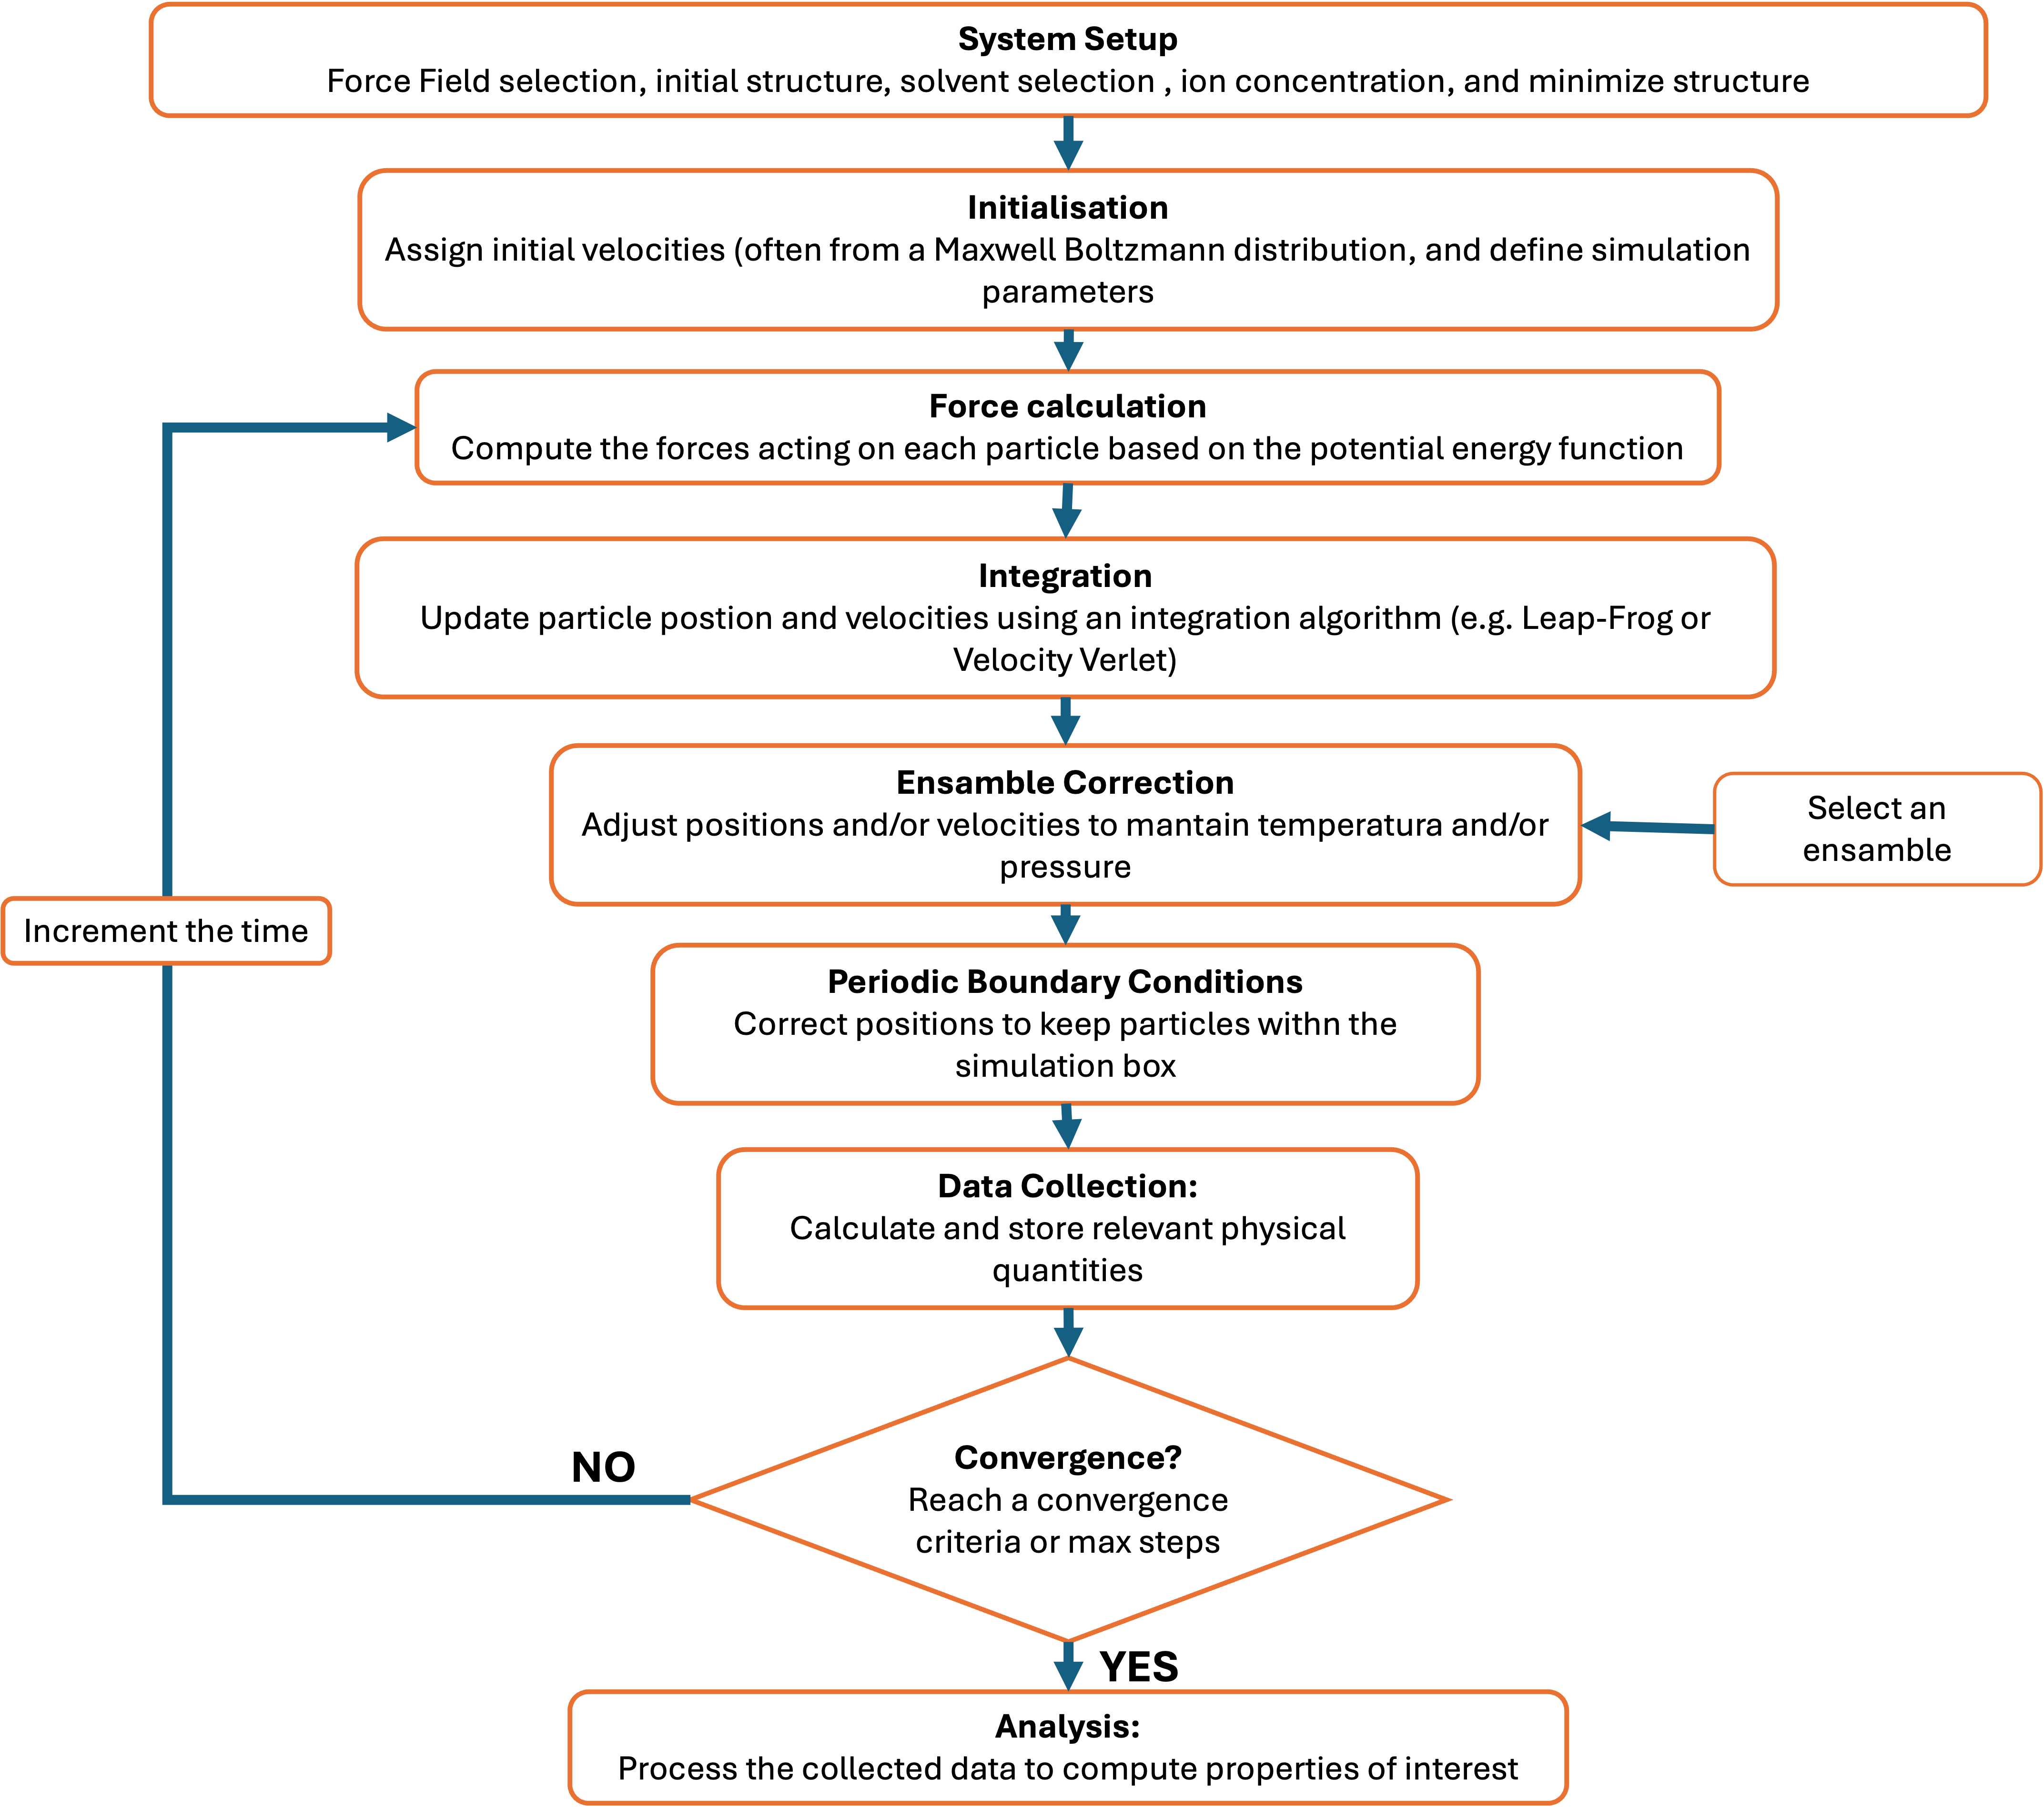
\includegraphics[width=1.0\linewidth]{General_Sections/Figures/MD_Workflow3.png}
    \caption{This scheme illustrates the essential steps involved in a MD simulation. The process begins with the definition of the initial state of the system, including the atomic coordinates and velocities, the selection of an appropriate force field, and the specification of the simulation conditions. The force field is then employed to compute the forces acting on each particle, which enables the time evolution of the system through the numerical integration of the equations of motion. At each time step, additional algorithms are applied to ensure that the system evolves under the desired thermodynamic conditions, such as constant temperature and/or pressure. This includes, for instance, the use of thermostats and barostats to control the corresponding ensemble. The propagation of positions and velocities, together with the enforcement of these conditions, is repeated iteratively over successive time steps. The simulation proceeds until a predefined convergence criterion is met or the maximum number of integration steps is reached.}
    \label{fig:MDFlow}
\end{figure}

The simulation process begins with system construction, including the selection of the force field, generation of the initial structure, solvent and ion setup, and energy minimization. Initial velocities are then assigned and simulation parameters are defined. At each time step, forces are computed from the potential energy function such as: 
\begin{equation}\label{NG}
    \vec{F_i} = - \vec{\nabla} U(\vec{r_{i}})
\end{equation}
Where $\vec{F}_i$ is the force acting on the $i$-th particle of the system, and $\vec{\nabla} U(\vec{r}_i)$ is the gradient of the potential energy function $U(\vec{r}_i)$, which is defined by a set of mathematical equations and parameters that collectively constitute a force field (FF). The selection of the FF is critical; it must faithfully reproduce the system's physical properties, as it governs the simulation's outcome~\cite{sereina,Conde2022}. Next, the position of the atoms are calculated by numerically integrating Newton's second law:
\begin{equation}\label{N2L}
    \vec{F}_i 
    = \frac{d\vec{p}_i}{dt}
    \xrightarrow{\text{constant }m_i}
    m_i \frac{d^2\vec{r}_i}{dt^2}
\end{equation}
where \(\vec{p}_i\), \(\vec{v}_i\) and \(m_i\) are the momentum, velocity, and mass of the \(i\)-th particle of the system, respectively, and \(t\) represents time. 
In a purely continuous and theoretical framework, the particle trajectory is
obtained by solving a second-order ordinary differential equation for the
position $\vec{r}_i(t)$, with time $t$ as the independent variable. Given an
initial position $\vec{r}_i(0)$ and velocity $\vec{v}_i(0)$, the state of the
system at any future time $t$ is determined by the solution of the equation
of motion:

\begin{equation}\label{eq:integral_v}
    \vec{v}_i(t) = \vec{v}_i(0) + \int_{0}^{t} \frac{\vec{F}_i(t')}{m_i} dt'
\end{equation}

\begin{equation}\label{eq:integral_r}
    \vec{r}_i(t) = \vec{r}_i(0) + \int_{0}^{t} \vec{v}_i(t') dt'
\end{equation}

However, because the force $\vec{F}_i$ acting on any single particle depends continuously on the ever-changing coordinates of all other interacting particles in the system, the integral in Equation~\ref{eq:integral_v} has no general analytical solution for a system of $N \geq 3$ particles. Consequently, evaluating the temporal evolution of the system requires shifting from a continuous analytical integration to a discrete numerical approximation.

This computational approach advances the simulation in finite, microscopic time increments, known as the time step ($\Delta t$). To achieve this, integration algorithms rely on the Taylor series expansion of the particle coordinates~\cite{braun2018best,biblia_2}. Mathematically, the Taylor series expansion of a general function $f(x)$ around a known point $a$ is expressed as:

\begin{equation}\label{eq:taylor_general}
    f(x) = f(a) + f'(a)(x-a) + \frac{f''(a)}{2!}(x-a)^2 + \frac{f'''(a)}{3!}(x-a)^3 + \dots
\end{equation}

By adapting this mathematical definition to the kinematics of a particle, the function becomes the position $\vec{r}_i$, the known point is the current time $t$, and the evaluated point is a small step forward in time ($t + \Delta t$). Consequently, the displacement $(x-a)$ corresponds to the time step $\Delta t$. Thus, the future position can be expanded as:

\begin{equation}\label{eq:taylor_forward}
    \vec{r}_i(t + \Delta t) = \vec{r}_i(t) + \vec{v}_i(t)\Delta t + \frac{1}{2}\vec{a}_i(t)\Delta t^2 + \frac{1}{6}\vec{j}_i(t)\Delta t^3 + \mathcal{O}(\Delta t^4)
\end{equation}
where $\vec{v}_i$ is the velocity (first derivative), $\vec{a}_i$ is the acceleration ($\vec{F}_i/m_i$, second derivative), $\vec{j}_i$ is the jerk (third derivative), and $\mathcal{O}(\Delta t^4)$ represents the local truncation error encompassing all higher-order terms. 

Similarly, to determine the position of the particle at the previous time step ($t - \Delta t$), we simply substitute $\Delta t$ with $-\Delta t$ in Equation~\ref{eq:taylor_forward}. Due to the alternating signs of the polynomial powers, this substitution yields:

\begin{equation}\label{eq:taylor_backward}
    \vec{r}_i(t - \Delta t) = \vec{r}_i(t) - \vec{v}_i(t)\Delta t + \frac{1}{2}\vec{a}_i(t)\Delta t^2 - \frac{1}{6}\vec{j}_i(t)\Delta t^3 + \mathcal{O}(\Delta t^4)
\end{equation}

By summing Equation~\ref{eq:taylor_forward} and Equation~\ref{eq:taylor_backward}, the odd-order derivatives (such as the velocity and the jerk) cancel out perfectly. Rearranging the result yields the classic Verlet integration algorithm~\cite{Verlet1967}:

\begin{equation}\label{eq:verlet}
    \vec{r}_i(t + \Delta t) = 2\vec{r}_i(t) - \vec{r}_i(t - \Delta t) + \frac{\vec{F}_i(t)}{m_i}\Delta t^2 + \mathcal{O}(\Delta t^4)
\end{equation}

Although the standard Verlet algorithm is computationally efficient and exhibits good numerical stability, it presents two important practical limitations. First, the position update involves the subtraction of two positions of similar magnitude, $2\vec{r}_i(t)-\vec{r}_i(t-\Delta t)$, which can lead to a loss of numerical precision due to floating-point round-off errors. Second, velocities do not explicitly enter the integration scheme and therefore must be estimated separately, typically from positions at adjacent time steps. This complicates the direct evaluation of the instantaneous kinetic energy and the application of temperature-control schemes based on the system's velocities.
To address these limitations, the \textit{leap-frog} integrator is widely used in molecular dynamics simulations and is the default integrator in the GROMACS simulation suite~\cite{leapfrog}. The leap-frog scheme is mathematically equivalent to the original Verlet algorithm, but reformulates the integration by evaluating velocities at half-integer time steps, $t\pm\frac{1}{2}\Delta t$, while positions are evaluated at integer time steps. The resulting staggered update of positions and velocities provides a more convenient representation of the system's dynamical state. The integration proceeds according to the following sequence:

\begin{equation}\label{eq:leapfrog}
    \begin{cases}
        \vec{v}_i(t+\frac{1}{2}\Delta t) = \vec{v}_i(t-\frac{1}{2}\Delta t) + \cfrac{\vec{F}_i(t)}{m_i} \Delta t \\
        \vec{r}_i(t+\Delta t) = \vec{r}_i(t) + \vec{v}_i(t+\frac{1}{2}\Delta t) \Delta t
    \end{cases}
\end{equation}
By structuring the integration in this staggered manner, the leap-frog scheme avoids the subtraction of large, closely spaced coordinate values present in the original Verlet formulation, thereby reducing the associated loss of numerical precision. At each time step, the forces acting on the particles are evaluated from the current configuration and used to update their velocities and positions. Repeated application of these equations generates the time evolution of the molecular system, providing the trajectory from which dynamical and thermodynamic properties can subsequently be calculated.

\paragraph{Constraint algorithms and the integration time step}

The selection of the integration time step is a critical factor governing the computational efficiency, numerical stability, and accuracy of MD simulations. Since the computational cost required to simulate a trajectory of a given physical duration increases as the time step decreases, using the largest stable $\Delta t$ is highly desirable~\cite{Conde2022}. However, the maximum allowable time step is constrained by the highest-frequency degrees of freedom in the system. To avoid numerical instability and limit integration errors, the time step must be sufficiently smaller than the period of the fastest internal motion, which typically corresponds to bond-stretching vibrations involving hydrogen atoms. Consequently, all-atom molecular systems without constraints typically require time steps of approximately 1~fs or smaller~\cite{Feenstra1999,Conde2022}.

To overcome this limitation and enable the use of larger integration time steps, constraint algorithms are routinely employed to remove selected high-frequency bond vibrations from the explicitly integrated degrees of freedom. In all-atom simulations, this commonly allows a time step of 2~fs to be employed. The SHAKE algorithm~\cite{shake_algorithm} was one of the earliest iterative methods developed to satisfy prescribed distance constraints. In modern GROMACS simulations, the parallel Linear Constraint Solver (LINCS) algorithm~\cite{lincs_algorithm} is widely used because of its computational efficiency and suitability for parallel implementations. Rather than iteratively solving the constrained equations of motion, LINCS determines the required corrections through a matrix-based linear constraint formulation. Additionally, because water molecules constitute a substantial fraction of the particles in biological systems, the analytical SETTLE algorithm~\cite{settle_algorithm} is specifically designed to enforce the rigid geometry of common water models, providing an efficient treatment of water constraints.

In the absence of external coupling, the underlying Newtonian equations of motion conserve the total energy of an isolated system. For a system with a fixed number of particles ($N$) and volume ($V$), the resulting dynamics therefore correspond to the microcanonical (\textit{NVE}) ensemble. In practice, however, numerical integration introduces small deviations from exact energy conservation, whose magnitude depends on the integration scheme and time step. Nevertheless, most biological processes in nature and experiments in the laboratory occur under approximately constant temperature ($T$) and/or pressure ($P$). Consequently, biomolecular simulations are frequently performed in the canonical (\textit{NVT}) or isothermal-isobaric (\textit{NPT}) ensembles~\cite{Frenkel2023,schlick2010molecular}. To reproduce these thermodynamic conditions, additional algorithms are introduced to couple the system to thermal and/or pressure reservoirs. Algorithms that regulate pressure are referred to as \textit{barostats}. They modify the dimensions and, consequently, the volume of the simulation cell according to the instantaneous pressure and the desired reference pressure. Several barostats are available for this purpose, including the stochastic cell-rescaling approach~\cite{CRB}. However, in the present work, only the Berendsen~\cite{BerendsenB} and Parrinello--Rahman~\cite{Parrinello1981} barostats were employed sequentially during equilibration and production simulations.

Similarly, algorithms that regulate temperature are referred to as \textit{thermostats}. These methods modify the kinetic degrees of freedom of the system to control its temperature. Depending on the algorithm, temperature regulation can be achieved through different mechanisms, including coupling the system to an external thermal bath or directly modifying the particle velocities. The latter principle underlies the velocity-rescaling thermostat employed in the present work~\cite{Vresc}.











































\subsection{Thermostats and barostats}

\paragraph{Statistical mechanics of temperature control}

According to the equipartition theorem, each degree of freedom contributes $k_B T / 2$ to the total energy, yielding the kinetic energy; $K = \frac{N_f}{2} k_B T$, where $N_f$ is the number of degrees of freedom and $k_B$ is the Boltzmann constant~\cite{nolting2018theoretical}. However, in a real system coupled to a thermal bath, the instantaneous kinetic energy is not strictly constant; it fluctuates. 

To determine the exact probability distribution of these macroscopic fluctuations, $P(K)$, we must first examine the system at the microscopic level. In the canonical (\textit{NVT}) ensemble, the probability of finding the system in one specific, exact microscopic state; defined by a unique set of individual momentum vectors $\{\vec{p}_i\}$; is governed strictly by the Boltzmann factor:

\begin{equation}
    P(\vec{p}_1, \vec{p}_2, \dots, \vec{p}_N) \propto e^{-K / k_B T_{\text{ref}}}
\end{equation}

However, in a macroscopic MD simulation, there are countless different ways to distribute the individual momenta among the particles that result in the exact same total $K$. To find the total probability of observing a macroscopic energy $K$, we must multiply the probability of a single microstate by the density of states, $\Omega(K)$~\cite{termo_metad_presion}. This crucial thermodynamic term quantifies the degeneracy of the system, representing the total number of microscopic momentum combinations that yield that exact total energy $K$:

\begin{equation}
    P(K) = \Omega(K) e^{-K / k_B T_{\text{ref}}}
\end{equation}

To mathematically determine this density of states $\Omega(K)$, we can use a geometric approach in phase space. Assuming for simplicity that all particles have the same mass $m$, the kinetic energy equation can be rewritten as $\sum_{i=1}^{N_f} p_i^2 = 2mK$, where $p_i$ represents each individual scalar momentum component. Mathematically, this equation perfectly matches the definition of the surface of an $N_f$-dimensional hypersphere, whose radius is $R = \sqrt{2mK} \propto K^{1/2}$. 

Geometrically, the surface area of such a hypersphere, and thus the number of available microstates $\Omega(K)$, scales as the radius raised to the power of the dimensions minus one ($R^{N_f - 1}$). Therefore, the density of states is proportional to~\cite{mec_estadistica}:

\begin{equation}
    \Omega(K) \propto (K^{1/2})^{N_f - 1} = K^{(N_f - 1)/2}
\end{equation}

 To express the final probability $P(K)$ in terms of the kinetic energy rather than momentum, a change of variables is required. Since $K \propto p^2$, the differentials relate as $dK \propto p\,dp$, which yields $dp \propto K^{-1/2} dK$. Combining the geometrical density of states with this differential change yields the final statistical weight:

\begin{equation}
    \Omega(K) \, dp \propto K^{(N_f - 1)/2} K^{-1/2} = K^{N_f/2 - 1}
\end{equation}

By incorporating this term into the macroscopic probability equation, the exact theoretical distribution of the kinetic energy in the \textit{NVT} ensemble is obtained as a Gamma distribution~\cite{gamma}:

\begin{equation}\label{eq:gamma_distribution}
    P(K) \propto K^{N_f/2 - 1} e^{-K / k_B T_{\text{ref}}}
\end{equation}

 By direct comparison\footnote{In probability theory, a Gamma distribution defined by a random variable $x$, a shape parameter $k$, and a scale parameter $\theta$ follows the proportionality $f(x) \propto x^{k-1} e^{-x/\theta}$.}, $K$ is the random variable, with shape parameter $k = N_f/2$ and scale parameter $\theta = k_B T_{\text{ref}}$. Its variance is therefore $\mathrm{Var}(K) = \frac{N_f}{2}(k_B T_{\text{ref}})^2$, which statistical mechanics dictates must be reproduced by any valid \textit{NVT} ensemble:

\begin{equation}\label{eq:variance_k}
    \sigma_K^2 = \langle K^2 \rangle - \langle K \rangle^2 = \frac{N_f}{2} (k_B T_{\text{ref}})^2
\end{equation}

Computationally, MD engines integrate Newton's equations of motion. In the absence of external coupling, these equations describe dynamics at constant total energy, corresponding to the microcanonical ($NVE$) ensemble, rather than the canonical ($NVT$) ensemble, in which the system exchanges energy with a thermal reservoir at a prescribed temperature. Thermostats introduce this coupling by modifying the particle dynamics to regulate the kinetic energy and thereby control the temperature. For velocity-rescaling thermostats, this is achieved through a scaling factor $\alpha$ applied to the particle velocities, while other thermostat families modify the equations of motion through different extended-system or stochastic formulations~\cite{BerendsenB,Vresc}. The physical behavior of rescaling-based thermostats therefore depends on how this scaling factor is determined.
The most rudimentary temperature-control scheme, known as \emph{simple velocity rescaling}, bypasses the natural thermodynamic fluctuations entirely. At each integration step, it forces the system to the exact target temperature by applying a rigid scaling factor defined as $\alpha = \sqrt{T_{\text{ref}}/T}$. 

To understand why this procedure is physically problematic, consider how this scaling factor affects the total kinetic energy. If every particle velocity is scaled according to $\vec{v}_i^{,\mathrm{new}} = \alpha \vec{v}_i$, the new total kinetic energy becomes:

\begin{equation}
K_{\mathrm{new}}
= \sum_{i=1}^{N} \frac{m_i(\alpha\vec{v}_i)\cdot(\alpha\vec{v}_i)}{2}
= \alpha^2 \sum_{i=1}^{N} \frac{m_i(\vec{v}_i\cdot\vec{v}_i)}{2}
= \alpha^2 K
\end{equation}
Substituting $\alpha^2 = T_{\mathrm{ref}}/T$ and using the proportionality between temperature and kinetic energy, $T_{\mathrm{ref}}/T = K_{\mathrm{ref}}/K$, gives:
\begin{equation}
K_{\mathrm{new}}
= \left(\frac{K_{\mathrm{ref}}}{K}\right)K
= K_{\mathrm{ref}}
\end{equation}
Thus, the instantaneous kinetic energy is forced to be identically equal to the target value at the end of every integration step. Consequently, its variance in the simulated system is zero, $\sigma_K^2=0$. A distribution with a fixed value and zero variance collapses mathematically to a Dirac delta function,
\begin{equation}
P_{\mathrm{simulated}}(K)
= \delta(K-K_{\mathrm{ref}})
\end{equation}
Simple velocity rescaling therefore imposes an isokinetic constraint rather than sampling the canonical ($NVT$) ensemble, eliminating the kinetic-energy fluctuations required for canonical sampling.


\paragraph{The Berendsen thermostat}

To avoid the unphysical abruptness of simple velocity rescaling, the
Berendsen thermostat introduces a gradual relaxation of the system towards
the target temperature over a specified relaxation time, $t_r$~\cite{BerendsenB}.
Since temperature is proportional to the instantaneous kinetic energy, this
relaxation can equivalently be expressed in terms of the kinetic energy $K$
as a first-order deterministic differential equation:

\begin{equation}\label{eq:berendsen_dk}
    \frac{dK}{dt}
    =
    \frac{K_{\mathrm{ref}}-K}{t_r}
\end{equation}

For a discrete integration time step $\Delta t$, the change in kinetic
energy is:

\begin{equation}
    \Delta K
    =
    (K_{\mathrm{ref}}-K)
    \frac{\Delta t}{t_r}
\end{equation}

Since the new kinetic energy is:

\begin{equation}
    K_{\mathrm{new}} = K + \Delta K
\end{equation}

and rescaling all particle velocities by a factor $\alpha$ changes the
kinetic energy according to:

\begin{equation}
    K_{\mathrm{new}} = \alpha^2 K
\end{equation}

the scaling factor can be obtained as:

\begin{equation}
    \alpha^2 K
    =
    K+
    (K_{\mathrm{ref}}-K)\frac{\Delta t}{t_r}
\end{equation}

which gives:

\begin{equation}
    \alpha
    =
    \sqrt{
        1+
        \frac{\Delta t}{t_r}
        \left(
            \frac{K_{\mathrm{ref}}}{K}-1
        \right)
    }
\end{equation}

Because the kinetic energy is proportional to the instantaneous temperature,
$K \propto T$, this expression can equivalently be written as:

\begin{equation}
    \alpha
    =
    \sqrt{
        1+
        \frac{\Delta t}{t_r}
        \left(
            \frac{T_{\mathrm{ref}}}{T}-1
        \right)
    }
\end{equation}

\paragraph{The stochastic v-rescale solution}

To circumvent the limitations of both simple rescaling (zero variance) and Berendsen (artificially restricted variance), Bussi, Donadio, and Parrinello introduced the stochastic velocity-rescaling algorithm (\textit{v-rescale})~\cite{Vresc}. Their crucial insight was to supplement the deterministic relaxation of the kinetic energy used in the Berendsen approach with an explicit stochastic contribution.
They redefined the evolution of the kinetic energy using a stochastic differential equation:


\begin{equation}\label{eq:vrescale}
    dK = \underbrace{(K_{\text{ref}} - K)\frac{dt}{t_r}}_{\text{Deterministic relaxation}} + \underbrace{2\sqrt{\frac{K K_{\text{ref}}}{N_f t_r}} dW}_{\text{Stochastic thermal noise}}
\end{equation}

The first term represents the deterministic relaxation of the kinetic energy towards its target value, analogous to the Berendsen thermostat. The second term introduces stochastic fluctuations through a Wiener process $dW$. The amplitude of this stochastic contribution is chosen such that, under the corresponding Fokker--Planck equation, the stationary distribution of the kinetic energy is the canonical Gamma distribution~\cite{Vresc}.

Consequently, the \textit{v-rescale} algorithm derives a stochastic scaling factor that ensures the stationary probability distribution of the kinetic energy converges to the theoretical Gamma distribution (Equation~\ref{eq:gamma_distribution}). This preserves the stable temperature relaxation of the Berendsen approach while correctly reproducing the thermodynamic fluctuations required to sample the canonical ($NVT$) ensemble~\cite{Vresc}.















\subsubsection{Statistical mechanics of pressure control}

To understand how barostats operate, it is first necessary to define how pressure is calculated at the microscopic level. In molecular simulations using Periodic Boundary Conditions (PBCs), there are no physical walls against which particles exert force. Instead, the instantaneous pressure is calculated from the microscopic virial expression. Because interactions can contribute differently along the three spatial directions ($X$, $Y$, and $Z$), pressure is generally represented by a $3\times3$ pressure tensor, $\mathbf{P}$, which contains kinetic and virial contributions~\cite{termo_metad_presion}:

\begin{equation}\label{eq:virial_tensor}
    \mathbf{P} = \frac{1}{V} \left( \underbrace{\sum_{i=1}^{N} \frac{\vec{p}_i \otimes \vec{p}_i}{m_i}}_{\text{Kinetic contribution}} - \underbrace{\sum_{i=1}^{N-1} \sum_{j=i+1}^{N} \vec{r}_{ij} \otimes \vec{f}_{ij}}_{\text{Virial contribution}} \right)
\end{equation}
where $V$ is the volume of the simulation cell, $\vec{p}_i$ is the momentum vector of particle $i$, $\vec{r}_{ij}$ is the displacement vector between two interacting particles, and $\vec{f}_{ij}$ is the force vector acting between them. The symbol $\otimes$ denotes the 
outer product of two vectors, yielding a second-order $3 \times 3$ tensor; explicitly, $(\vec{a} \otimes \vec{b})_{ij} = a_i b_j$. For an isotropic system, the scalar pressure is obtained as one-third of the trace of the pressure tensor: $p = \text{Tr}(\mathbf{P})/3$.

In an $NVT$ simulation, the volume is fixed, while the instantaneous pressure fluctuates as the particles move. In an $NPT$ simulation, the volume of the simulation cell is allowed to fluctuate around a value consistent with a prescribed reference pressure, $\mathbf{P}_{\mathrm{ref}}$. Depending on the pressure-coupling scheme, the shape of the simulation cell may also be allowed to fluctuate. In pressure-coupling schemes based on cell rescaling, pressure deviations are compensated by applying a scaling transformation to the simulation cell and the particle coordinates. A general rescaling can be represented by a transformation matrix $\mathbf{M}$ acting on the particle coordinates and the simulation-cell volume:

\begin{subequations}\label{eq:scaling_general}
    \begin{align}
        \vec{x} &\rightarrow \mathbf{M}\vec{x} \\
        V &\rightarrow \det(\mathbf{M})V
    \end{align}
\end{subequations}

Here, $\mathbf{M}$ determines the deformation applied to the simulation cell, including changes in its dimensions and, for anisotropic coupling, its shape. The specific form of this transformation depends on the pressure-coupling scheme.


\paragraph{The Berendsen barostat}
The Berendsen barostat provides a simple and stable procedure for relaxing the simulation box towards a prescribed reference pressure~\cite{BerendsenB}. Its underlying principle is that deviations between the instantaneous pressure and the reference pressure induce a gradual change in the dimensions of the simulation box. The magnitude of this response depends on the pressure difference, the isothermal compressibility of the system, and the chosen pressure-relaxation time $t_r$.
For the Berendsen scheme, the scaling matrix can be written as:
\begin{equation}\label{eq:berendsen}
\mathbf{M}
=
\mathbb{I}
-
\frac{\Delta t}{3t_r}
\boldsymbol{\beta}
\odot
\left(
\mathbf{P}
-
\mathbf{P}_{\mathrm{ref}}
\right)
\end{equation}
where $\Delta t$ is the integration timestep, $\boldsymbol{\beta}$ is the isothermal compressibility tensor, and $\odot$ denotes the Hadamard
(element-wise) product. Here, $\mathbb{I}$ represents the identity transformation, while the pressure difference
$\mathbf{P}-\mathbf{P}_{\mathrm{ref}}$ determines the magnitude of the box deformation, with different components contributing independently in anisotropic coupling. The compressibility determines the response of the system to a pressure difference, while the relaxation time
$t_r$ controls the rate of the response.

For isotropic pressure coupling, a common scaling factor is applied to the three spatial dimensions. In anisotropic or semi-isotropic coupling, the corresponding components of the pressure and compressibility tensors determine how the individual box dimensions are scaled. The scaling is therefore applied gradually over successive integration steps rather than enforcing an instantaneous pressure correction.
An important limitation of the Berendsen barostat is that the deterministic rescaling suppresses the magnitude of the natural fluctuations of the simulation cell. Consequently, although it provides efficient pressure relaxation, it does not generate the correct volume fluctuations of the isothermal-isobaric ensemble~\cite{BerendsenB}.

\paragraph{The stochastic cell-rescaling (C-rescale) barostat}
The stochastic cell-rescaling (C-rescale) barostat is a stochastic variant of the Berendsen pressure-coupling scheme that allows the correct equilibrium volume fluctuations to be sampled~\cite{CRB}. As in the Berendsen approach, the simulation coordinates and box vectors are rescaled at regular intervals, producing a first-order relaxation of the pressure towards a prescribed reference pressure. The difference is that the rescaling includes a stochastic contribution that restores the equilibrium volume fluctuations.
For isotropic pressure coupling, the volume evolution can be expressed in terms of the volumetric strain $\epsilon=\log(V/V_0)$ as~\cite{CRB,Gromacs2015}:
\begin{equation}\label{eq:crescale}
d\epsilon
=
-\frac{\beta}{t_r}
\left(
P_{\mathrm{ref}}-P
\right)dt
+
\sqrt{
\frac{2k_BT\beta}{Vt_r}
}\,dW
\end{equation}
where $\beta$ is the isothermal compressibility, $t_r$ is the pressure-relaxation time, $V$ is the instantaneous simulation-cell volume, and $dW$ represents an increment of a Wiener process. The first term describes the deterministic relaxation of the pressure towards the reference pressure, analogous to the Berendsen scheme, whereas the second term introduces stochastic fluctuations into the cell-rescaling process.
Unlike the deterministic Berendsen barostat, the stochastic contribution allows C-rescale to reproduce the correct equilibrium volume fluctuations of the $NPT$ ensemble while retaining a first-order pressure-relaxation behavior~\cite{CRB}.

\paragraph{The Parrinello--Rahman barostat}
The Parrinello--Rahman approach differs fundamentally from direct cell-rescaling methods because the simulation cell itself is treated as a set of additional dynamical degrees of freedom~\cite{Parrinello1981}. Rather than prescribing an instantaneous scaling factor, the method introduces an extended Lagrangian in which the cell vectors evolve dynamically in response to the difference between the instantaneous and reference pressure tensors.
Let $\mathbf{L}$ denote the cell matrix, whose columns are the three vectors defining the simulation cell. In the Parrinello--Rahman formulation, the cell dynamics can be written schematically as:
\begin{equation}\label{eq:parrinellorahman1}
\ddot{\mathbf{L}}
=
V\mathbf{W}^{-1}
\left(\mathbf{L}^{\mathrm{T}}\right)^{-1}
\left(
\mathbf{P}
-
\mathbf{P}_{\mathrm{ref}}
\right)
\end{equation}
where $V$ is the simulation-cell volume and $\mathbf{W}$ is a matrix parameter that controls the inertial response of the simulation cell~\cite{Gromacs2015}. Thus, deviations between the instantaneous and reference pressure tensors drive the dynamical deformation of the simulation cell.
Because the simulation cell evolves dynamically, its deformation is also coupled to the particle motion. Consequently, the equations of motion are modified to account for the time-dependent geometry of the simulation cell. By treating the simulation cell as a dynamical degree of freedom, the Parrinello--Rahman method allows the system to reproduce the correct equilibrium fluctuations of the isothermal-isobaric ($NPT$) ensemble.
However, the dynamical response of the cell can lead to pronounced oscillations when the system is far from the target pressure. Therefore, Parrinello--Rahman coupling is generally more appropriate after an initial equilibration stage, when the pressure and volume are already reasonably close to their target values.




\paragraph{Comparison and application of pressure coupling methods}

The three barostats considered here differ in their treatment of pressure relaxation and volume fluctuations, making them suitable for different stages of an MD simulation. The Berendsen barostat provides stable and rapid relaxation towards the target pressure, which makes it useful during the initial equilibration of the system. However, because it suppresses the natural pressure and volume fluctuations, it does not sample the correct $NPT$ ensemble. In contrast, the Parrinello--Rahman barostat allows the system to sample the appropriate equilibrium fluctuations, but can exhibit substantial box oscillations when applied to systems that are far from mechanical equilibrium. It is therefore generally more suitable after an initial equilibration stage. The stochastic cell-rescaling (C-rescale) barostat combines pressure relaxation with stochastic fluctuations, allowing the correct equilibrium volume fluctuations to be reproduced while maintaining stable pressure relaxation~\cite{Gromacs2015,CRB}.
In the MD simulations presented in this thesis, the Berendsen barostat was therefore employed during the initial equilibration stages to allow the system volume to relax smoothly towards the target pressure, followed by Parrinello--Rahman during the production simulations to obtain the appropriate thermodynamic fluctuations.




\paragraph{Semi-isotropic pressure coupling: Preserving membrane integrity}
Lipid bilayers are mechanically anisotropic systems, with their response to pressure differing substantially between the membrane plane and the direction normal to it. Consequently, pressure coupling in membrane simulations requires the lateral ($XY$) and normal ($Z$) dimensions of the simulation box to be treated differently.
Under isotropic pressure coupling, the three box dimensions are coupled to the same pressure response. Such scaling is appropriate for approximately isotropic systems, but is generally not suitable for lipid bilayers because the membrane exhibits different mechanical responses in the lateral and normal directions. In contrast, semi-isotropic pressure coupling couples the two lateral dimensions, $X$ and $Y$, while treating them independently from the normal dimension, $Z$.
Thus, the lateral dimensions are scaled together to preserve the symmetry of the membrane plane, whereas the normal dimension is allowed to respond independently to the pressure along the membrane normal. This can be represented by a compressibility tensor of the form:
\begin{equation}
\begin{pmatrix}
\beta_{xy} & 0 & 0 \\
0 & \beta_{xy} & 0 \\
0 & 0 & \beta_z
\end{pmatrix}
\end{equation}
where $\beta_{xy}$ describes the common compressibility applied to the two lateral directions, while $\beta_z$ describes the response along the membrane normal.
This separation allows the membrane area to equilibrate independently from the box dimension normal to the bilayer, providing an appropriate treatment of the distinct lateral and normal responses of the membrane. The choice of pressure-coupling scheme can influence the structural and dynamical properties of lipid bilayers and should therefore be considered carefully in membrane simulations~\cite{Ivanova2018,Gromacs2015,10.1371/journal.pcbi.1000810}























































\subsection{Periodic boundary conditions}
Nevertheless, despite the thermodynamic control offered by these algorithms, the simulation of real-world systems is limited by the amount of particles that can be simulated using a realistic amount of computational resources. This limitation necessitates confining the molecules to a finite volume; however, enclosing them with hard boundaries would introduce artificial particle-wall interactions that are unrealistic for biological environments. To avoid this, when the calculation of the new positions displaces a particle out of the simulation cell, the exact same particle wraps around and re-enters from the opposite side.

This approach effectively models an infinite system by tiling the simulation cell in all directions of space, creating periodic replicas where every particle is and behaves exactly like its original counterpart. This method is depicted in Figure~\ref{fig:PBCs}, and when applied, the system is said to be under PBCs. When applying this method, the simulation box must be large enough to avoid any possible interactions between replicas of the same molecule~\cite{braun2018best}.
\begin{figure}[!htbp]
    \centering
    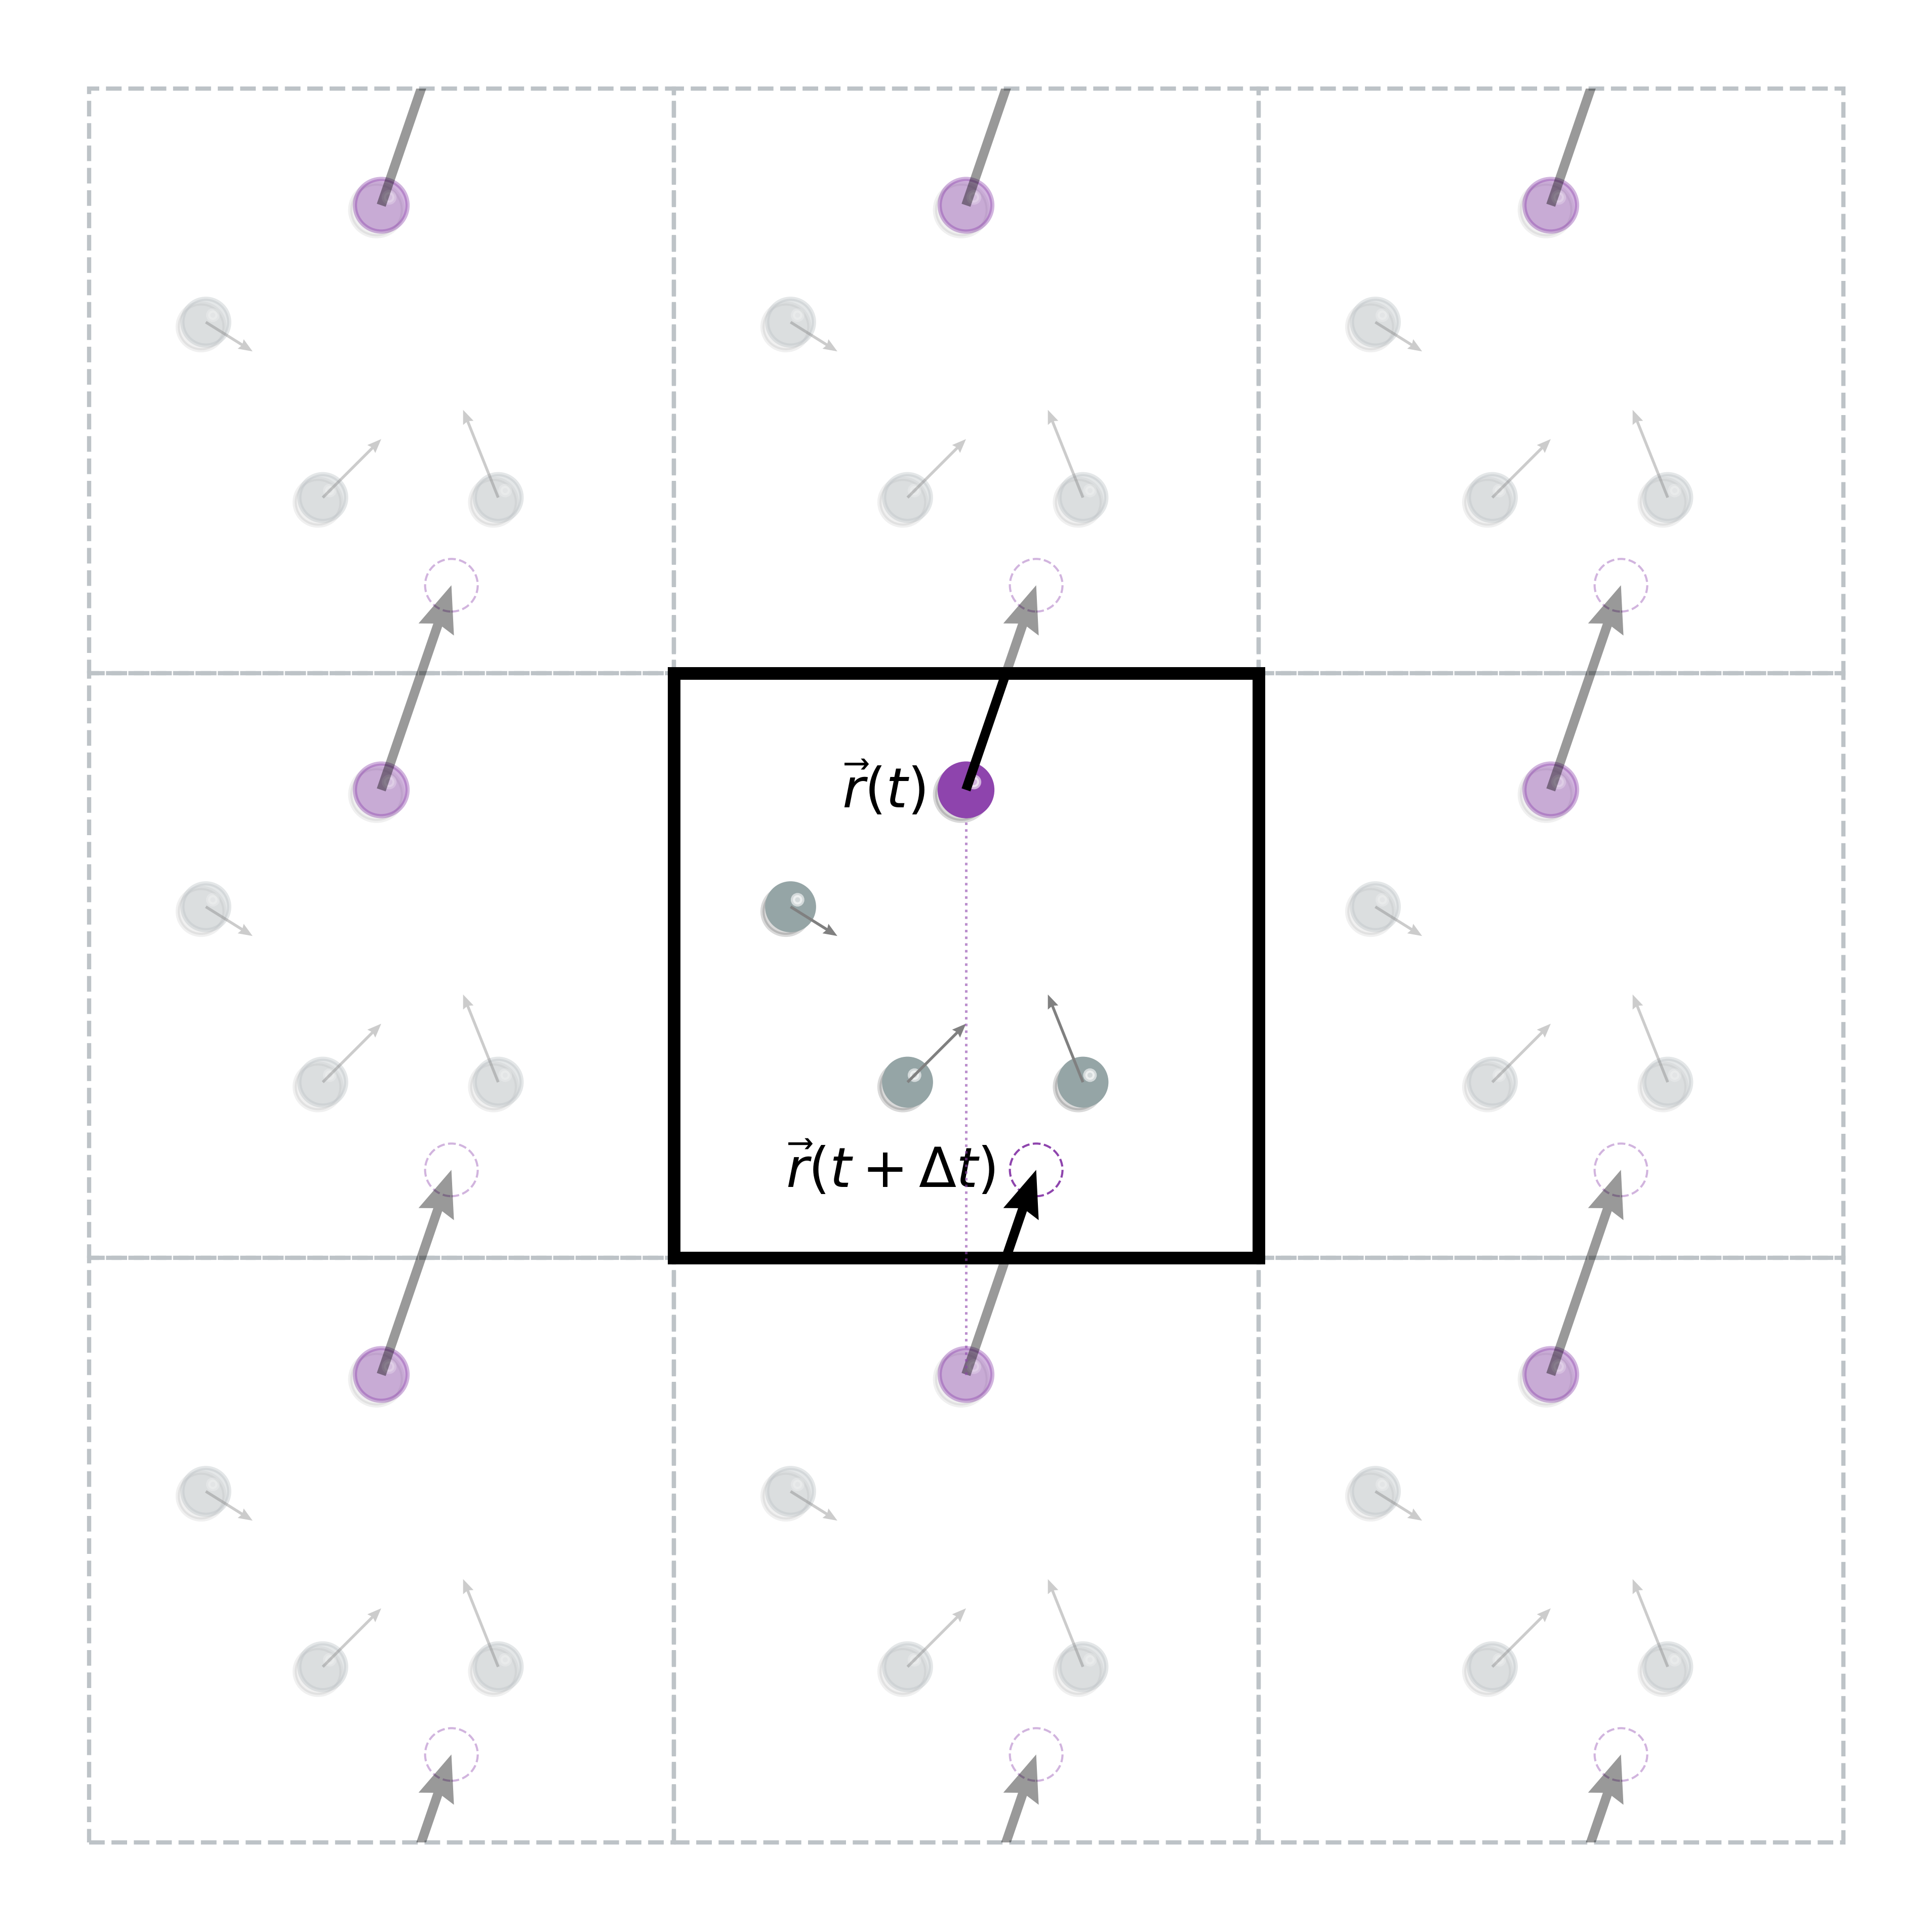
\includegraphics[width=0.55\linewidth]{General_Sections/Figures/pbc_diagram.png}
    \caption{Scheme depicting the effect of PBCs. The image shows how a particle that at an instant \(t\) is displaced outside the original simulation space (black solid line), re-enters into the box from its periodic image at a time \(t + \Delta t\). The number of particles in the simulation cell and in all the periodic images are kept constant. Image generated with Matplotlib.}
    \label{fig:PBCs}
\end{figure}
In the final step of the MD workflow shown in Figure~\ref{fig:MDFlow}, the MD engine writes the new positions, velocities, thermodynamic properties, and other relevant data into output files. If a convergence criterion is met or a user-defined number of steps are completed, the simulation finishes, allowing for subsequent qualitative and quantitative analysis. As noted above, the results obtained depend on the force field selected, as it governs the interactions between particles. The following section examines the general structure of force fields, with particular emphasis on the different contributions to the potential function used to compute the forces acting on each particle.


\subsection{Force fields}

A force field is a set of equations and parameters used to describe the potential energy of a molecular system and, consequently, the interactions between its particles. In general, the potential energy function can be decomposed into bonded and non-bonded contributions:

\begin{equation}
U(\vec{r}) =
U_{\mathrm{bonded}}(\vec{r}) +
U_{\mathrm{non-bonded}}(\vec{r})
\end{equation}

\subsubsection{Bonded interactions}
The bonded term describes interactions between particles whose relative positions are constrained by the molecular connectivity of the system. These interactions are defined by the covalent topology and account for local structural degrees of freedom, including bond stretching, angle bending, and torsional motions. The bonded contribution to the potential energy can be decomposed as:
\begin{equation}
U_{\mathrm{bonded}}(\vec{r}) =
U_{\mathrm{bonds}}(\vec{r}) +
U_{\mathrm{angles}}(\vec{r}) +
U_{\mathrm{proper\ dihedrals}}(\vec{r}) +
U_{\mathrm{improper\ dihedrals}}(\vec{r})
\end{equation}



The bond-stretching contribution describes the variation in distance between two covalently connected particles (Fig.~\ref{fig:bond_stretching}), whereas the angle-bending contribution accounts for variations in the angle formed by three consecutively connected particles (Fig.~\ref{fig:angle_bending}). Torsional contributions involve four particles and describe rotations about the corresponding molecular bonds. These are commonly divided into proper dihedrals, which describe torsion around a sequence of four consecutively connected particles (Fig.~\ref{fig:dihedral_proper}), and improper dihedrals, which constrain the relative geometry of four particles and are commonly used to maintain planarity or stereochemical configurations (Fig.~\ref{fig:dihedral_improper}).
\begin{figure}[!htb]
\centering

\begin{subfigure}[b]{0.48\linewidth}
    \centering
    
\includegraphics[width=0.95\linewidth]{bonded_interactions/bond_stretching.pdf}
    \caption{Bond stretching}
    \label{fig:bond_stretching}
\end{subfigure}
\hfill
\begin{subfigure}[b]{0.48\linewidth}
    \centering
    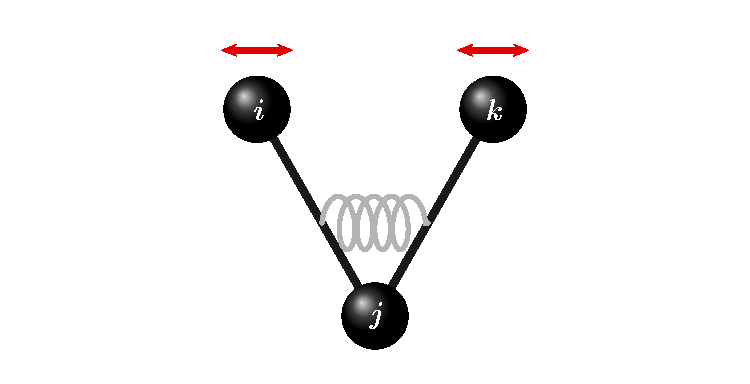
\includegraphics[width=0.95\linewidth]{bonded_interactions/angle_bending.pdf}
    \caption{Angle bending}
    \label{fig:angle_bending}
\end{subfigure}

\vspace{2ex}

\begin{subfigure}[b]{0.48\linewidth}
    \centering
    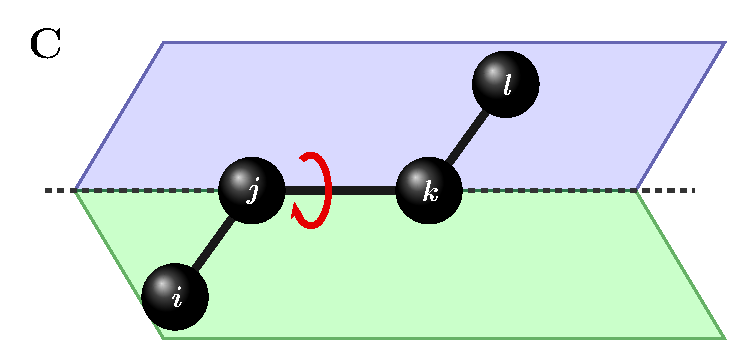
\includegraphics[width=0.95\linewidth]{bonded_interactions/dihedral_proper.pdf}
    \caption{Proper dihedral}
    \label{fig:dihedral_proper}
\end{subfigure}
\hfill
\begin{subfigure}[b]{0.48\linewidth}
    \centering
    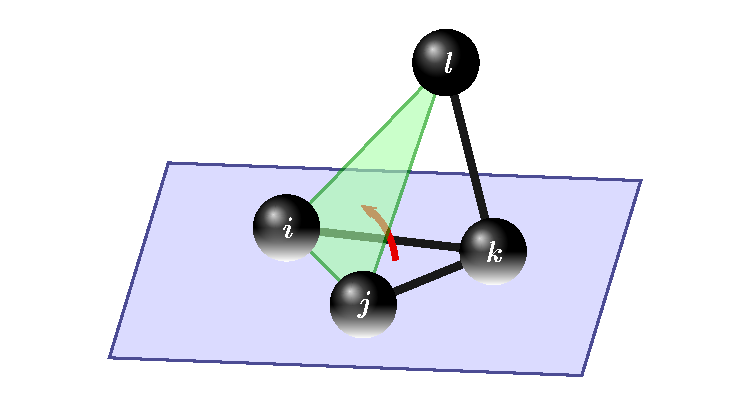
\includegraphics[width=0.95\linewidth]{bonded_interactions/dihedral_improper.pdf}
    \caption{Improper dihedral}
    \label{fig:dihedral_improper}
\end{subfigure}

\caption{Schematic representation of the bonded interactions included in the bonded term of the potential function. (a) Bond stretching between two covalently connected particles, (b) angle bending involving three consecutively connected particles, (c) torsion about a proper dihedral angle involving four consecutively connected particles, and (d) an improper dihedral used to control the relative arrangement of four particles.}
\label{fig:FF_bonded}

\end{figure}
Bond and angle terms are commonly represented using harmonic potentials:
\begin{equation}
U_{\mathrm{bonds}}(\vec{r}_{ij}) =
\frac{1}{2} k_{ij}
\left(
\vec{||r_{ij}||} - r_{ij}^{0}
\right)^2
\end{equation}

\begin{equation}
U_{\mathrm{angles}}(\theta_{ijk}) =
\frac{1}{2} k_{ijk}
\left(
\theta_{ijk} - \theta_{ijk}^{0}
\right)^2.
\label{eq:angle}
\end{equation}

Here, $\vec{r}_{ij}$ denotes the instantaneous distance between particles $i$ and $j$, whereas $r_{ij}^{0}$ is the corresponding equilibrium bond distance and $k_{ij}$ is the associated force constant. Similarly, $\theta_{ijk}$ is the instantaneous angle formed by particles $i$, $j$, and $k$, $\theta_{ijk}^{0}$ is its equilibrium value, and $k_{ijk}$ is the corresponding force constant. The values of these equilibrium geometries and force constants are determined by the specific force field and molecular topology.

The torsional contribution accounts for the rotational degrees of freedom associated with four connected particles. A common functional form for proper dihedrals is a periodic potential,
\begin{equation}
U_{\mathrm{proper\ dihedral}}(\phi_{ijkl}) =
k_{ijkl}
\left[
1 + \cos
\left(
n\phi_{ijkl} - \phi_{ijkl}^{0}
\right)
\right]
\end{equation}
where $\phi_{ijkl}$ is the instantaneous dihedral angle defined by particles $i$, $j$, $k$, and $l$, $n$ is the periodicity or multiplicity of the torsional potential, $k_{ijkl}$ is the corresponding force constant, and $\phi_{ijkl}^{0}$ is the phase offset. Unlike the bond and angle terms, which are typically associated with a single equilibrium geometry, the periodic form of the proper dihedral potential can represent multiple energetically preferred conformations.

Improper dihedrals are generally introduced to control the relative geometry of four particles and are commonly used to maintain planarity or a particular stereochemical configuration. A harmonic functional form is frequently employed:
\begin{equation}
U_{\mathrm{improper\ dihedral}}(\xi_{ijkl}) =
\frac{1}{2} k_{ijkl}
\left(
\xi_{ijkl} - \xi_{ijkl}^{0}
\right)^2
\end{equation}
Here, $\xi_{ijkl}$ denotes the instantaneous improper dihedral angle, $\xi_{ijkl}^{0}$ is its reference value, and $k_{ijkl}$ is the associated force constant. As for the bond and angle terms, both the reference value and the force constant are parameters defined by the particular force field.

Together, these bonded contributions provide the energetic description of the internal molecular geometry imposed by the force-field topology. Their functional forms and associated parameters determine how strongly deviations from the preferred bond lengths, bond angles, and torsional configurations are penalized.




\subsubsection{Non-bonded interactions}
The non-bonded term of the potential function accounts for van der Waals and electrostatic interactions between particle pairs that are not treated explicitly as bonded interactions. Under PBCs, these interactions extend beyond the primary simulation box and include interactions with the periodic images of other particles. The treatment of these periodic interactions is therefore an essential aspect of molecular dynamics simulations~\cite{braun2018best}.
The non-bonded potential is typically decomposed into two main contributions, namely van der Waals (vdW) and electrostatic interactions:
\begin{equation}
U_{\mathrm{non-bonded}}(\vec{r}) =
U_{\mathrm{vdW}}(\vec{r}) +
U_{\mathrm{electrostatic}}(\vec{r})
\end{equation}
If all pairwise interactions were evaluated explicitly, the computational cost would scale as $\mathcal{O}(N^2)$. This scaling becomes prohibitive for systems containing thousands or millions of particles. Efficient MD algorithms therefore exploit the different spatial decay properties of the two contributions and introduce suitable approximations or specialized algorithms to reduce the computational cost while retaining the relevant physical interactions~\cite{braun2018best,Gromacs2015,Frenkel2023}
Throughout this section, the term \textit{particle} is used rather than \textit{atom}, since the interacting units depend on the resolution of the force field. In atomistic models, a particle generally corresponds to an individual atom, whereas in coarse-grained models a particle may represent a group of atoms. The parameters defining the non-bonded interactions, such as partial charges and van der Waals parameters, are force-field-specific and are commonly obtained by fitting to experimental data, quantum-mechanical calculations, or a combination of both. Some force fields may additionally include \textit{cross terms} that couple different contributions to the potential energy, providing a more detailed description of the system at the expense of increased model complexity~\cite{cross_term}.



\subsubsubsection{Van der Waals interactions and truncation methods}
The van der Waals contribution accounts for short-range attractive and repulsive interactions between particles. A common representation is the Lennard--Jones potential, which combines a short-range repulsive term with a longer-range attractive dispersion term:
\begin{equation}
U_{\mathrm{vdW}}(\vec{r}_{ij})
=
4\epsilon_{ij}
\left[
\left(\frac{\sigma_{ij}}{r_{ij}}\right)^{12}
-
\left(\frac{\sigma_{ij}}{r_{ij}}\right)^{6}
\right]
\end{equation}
where $r_{ij}=||\vec{r}_i-\vec{r}_j||$ is the distance between particles $i$ and $j$, $\epsilon_{ij}$ determines the depth of the potential well, and $\sigma_{ij}$ is the distance at which the potential is zero (i.e., the effective particle diameter).
Because the attractive dispersion term of the Lennard--Jones potential decays as $r^{-6}$, its contribution decreases rapidly with increasing
distance. In practical MD simulations, the calculation is therefore commonly truncated at a finite cutoff distance $r_c$. Particle pairs separated by distances greater than $r_c$ are not evaluated explicitly, substantially reducing the computational cost compared with an exhaustive pairwise calculation.
A simple truncation of the potential, however, introduces a discontinuity at the cutoff. Depending on the treatment employed, this can lead to discontinuous energies or forces and consequently to numerical artifacts. To alleviate this problem, the potential or force can be modified in the vicinity of the cutoff. For example, a potential-shift scheme shifts the potential so that it vanishes at $r_c$, whereas a force-switch scheme smoothly reduces the force to zero over a specified switching interval~\cite{termo_metad_presion}. To account for the contribution of van der Waals interactions beyond the cutoff, analytical long-range corrections to the energy and pressure are commonly applied under the assumption that the radial distribution function is unity for $r > r_c$~\cite{braun2018best}.

\subsubsubsection{Electrostatic interactions and long-range solvers}
The electrostatic contribution describes the interactions between charged
particles and is commonly represented by Coulomb's law:
\begin{equation}
U_{\mathrm{electrostatic}}(\vec{r}_{ij})
=
\frac{1}{4\pi\varepsilon_0}
\frac{q_iq_j}{\varepsilon_r r_{ij}}
\end{equation}
where $q_i$ and $q_j$ are the partial charges of particles $i$ and $j$,
$r_{ij}$ is their separation distance, $\varepsilon_0$ is the vacuum
permittivity, and $\varepsilon_r$ is the relative permittivity. In
classical force fields, the partial charges are typically fixed force-field parameters.
Unlike the van der Waals contribution, the Coulomb potential decays as $r^{-1}$ and therefore remains significant over much longer distances.
Consequently, applying a simple cutoff to electrostatic interactions can introduce substantial artifacts by neglecting long-range contributions.
Specific methods are therefore required to treat long-range
electrostatic interactions, particularly under PBCs.

\paragraph{Reaction Field}
One approach to account approximately for long-range electrostatic effects is the Reaction Field method. It assumes that the region beyond the cutoff distance $r_c$ can be represented as a homogeneous dielectric medium with relative permittivity $\varepsilon_{\mathrm{RF}}$. Within the cutoff region, the modified electrostatic potential can be written as~\cite{reaction_field}:
\begin{equation}\label{eq:reactionfield}
U_{\mathrm{RF}}(\vec{r}_{ij}) =
\frac{1}{4\pi\varepsilon_0}
\frac{q_iq_j}{\varepsilon_r}
\left[\frac{1}{r_{ij}}+\frac{\varepsilon_{\mathrm{RF}}-\varepsilon_r}{2\varepsilon_{\mathrm{RF}}+\varepsilon_r}
\frac{r_{ij}^{2}}{r_c^{3}}-\frac{1}{r_c}
\frac{3\varepsilon_{\mathrm{RF}}}{2\varepsilon_{\mathrm{RF}}+\varepsilon_r}
\right]
\end{equation}
The constant term is chosen such that the potential vanishes at the cutoff distance. In addition, the reaction-field correction causes the derivative of the potential, and therefore the force, to vanish at $r_c$. This provides a smoother truncation than a simple Coulomb cutoff.
However, the method relies on the assumption that the environment beyond the cutoff can be represented by a homogeneous dielectric medium, which may be inappropriate for heterogeneous systems such as biological membranes~\cite{termo_metad_presion}.
\paragraph{Ewald summation and Particle-Mesh Ewald (PME)}
A more rigorous treatment of long-range electrostatics under PBCs is provided by Ewald summation. The electrostatic energy of a periodic system can be formally expressed as an infinite sum over all periodic images:
\begin{equation}\label{eq:coulomb_periodic}
    U_{\text{Coulomb}}(\vec{r}_{ij}) = \frac{1}{4\pi\varepsilon} \sum_{\vec{n}^*} \frac{1}{2} \sum_{i=1}^{N} \sum_{j=1}^{N} \frac{q_i q_j}{\|\vec{r}_{ij} + \vec{n}\|}
\end{equation}

where $\vec{n}^*$ is a periodic lattice vector and the asterisk indicates that the self-interaction term with $i=j$ and $\vec{n}=\vec{0}$ is excluded. This sum is conditionally convergent and converges very slowly,
making its direct evaluation computationally inefficient~\cite{Ewald1921,Frenkel2023}.
Ewald summation overcomes this difficulty by introducing a Gaussian screening distribution around each point charge. The resulting expression can be decomposed into rapidly converging direct-space and reciprocal-space terms, together with a self-energy correction~\cite{pme}:

\begin{equation}\label{eq:ewald_total}
\begin{aligned}
    U_{\text{Coulomb}}(\vec{r}_{ij}) &= \underbrace{ \frac{1}{4\pi\varepsilon} \sum_{\vec{n}^*} \frac{1}{2} \sum_{i=1}^{N} \sum_{j=1}^{N} \frac{q_i q_j \text{erfc}(\beta\|\vec{r}_{ij} + \vec{n}\|)}{\|\vec{r}_{ij} + \vec{n}\|} }_{\text{Direct Space}} \\
    &+ \underbrace{ \frac{1}{4\pi\varepsilon \pi V} \sum_{\vec{m}^*} \frac{1}{2} \sum_{i=1}^{N} \sum_{j=1}^{N} \frac{q_i q_j e^{-(\pi\vec{m}/\beta)^2} e^{i 2\pi\vec{m}\cdot\vec{r}_{ij}}}{\|\vec{m}\|^2} }_{\text{Reciprocal Space}} \\
    & - \underbrace{ \frac{1}{4\pi\varepsilon} \frac{\beta}{\sqrt{\pi}} \sum_{i=1}^{N} q_i^2 }_{\text{Self-Energy Correction}}
\end{aligned}
\end{equation}

Here, $\beta$ is a parameter that controls the width of the Gaussian charge distribution. The Ewald formulation separates the electrostatic energy into three contributions. The direct-space term decays rapidly due to the complementary error function ($\text{erfc}$), allowing it to be truncated beyond a defined real-space cutoff. The reciprocal-space term accounts for the long-range electrostatic interactions between the periodic images and is evaluated in Fourier space over the wave vectors $\vec{m}$. Finally, a self-energy correction is included to remove the artificial interaction between each charge and its own Gaussian distribution.


The standard Ewald summation provides an accurate treatment of long-range electrostatic interactions, but its computational cost becomes limiting for large molecular systems. To overcome this limitation, the Particle Mesh Ewald (PME) method was introduced~\cite{Frenkel2023,Darden1993,pme}. In PME, the reciprocal-space contribution is calculated on a regular three-dimensional grid using Fast Fourier Transforms (FFT), which makes the calculation considerably more efficient~\cite{pme}. PME is therefore widely used in modern molecular dynamics simulations to efficiently account for long-range electrostatic interactions.



\begin{figure}[!htbp]
    \centering
    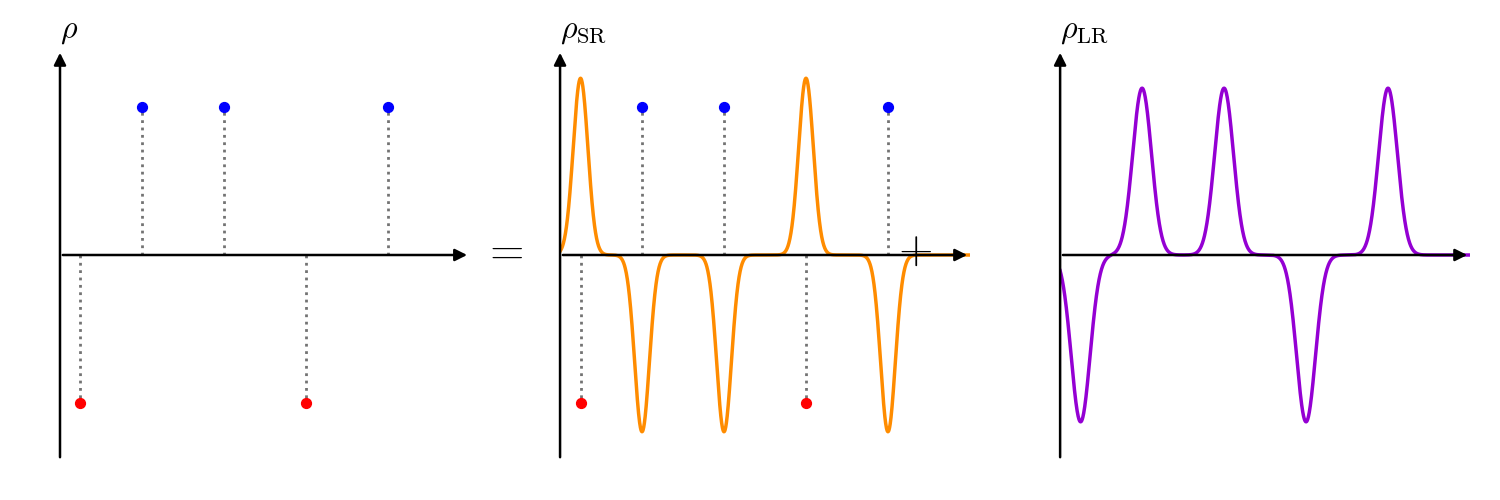
\includegraphics[width=1\linewidth]{General_Sections/Figures/pme.png}
    \caption{Charge distribution in the particle-mesh Ewald method. \textbf{(Left)} The charge density of point particles is that of a Dirac delta located in the position of the particle. The decomposition of the short and long-range contributions are equivalent to have \textbf{(center)} in the direct space the same distribution of Dirac-like charge density and a complementary Gaussian distribution, in the same position and with the same charge but opposite sign; and \textbf{(right)} Gaussian distribution of charges, with the same sign and magnitude as the original, in the reciprocal space. This treatment allows for a rapid convergence of the series, while keeping the periodicity of the system.}
    \label{fig:pme}
\end{figure}























\subsection{Force field resolution}

Force fields can be broadly classified according to their level of resolution, that is, according to how the molecular structure is represented and which atoms are treated as individual interaction sites. At the highest resolution are atomistic or all-atom (AA) force fields, such as Chemistry at Harvard Macromolecular Mechanics (CHARMM)~\cite{charmm}, Assisted Model Building with Energy Refinement (AMBER)~\cite{gaff}, and the Optimized Potentials for Liquid Simulations (OPLS) family~\cite{oplsaa}. In these models, atoms are represented explicitly, including hydrogen atoms. This level of resolution provides access to detailed structural and interaction features, which can be important when the phenomenon of interest depends on specific atomic interactions. However, the greater number of degrees of freedom also increases the computational cost of the simulations, particularly for systems containing large numbers of solvent molecules or extended assemblies such as lipid membranes. Although the direct evaluation of pairwise interactions would formally scale as $\mathcal{O}(N^2)$, practical MD implementations reduce this cost through techniques such as neighbor lists for short-range interactions and particle-mesh methods for long-range electrostatics~\cite{kim2023neighbor,pme}. The computational effort therefore depends not only on the number of particles, but also on the simulation algorithm, hardware, system size, and sampling protocol. Consequently, the accessible spatial and temporal scales of AA simulations are system-dependent and must be considered together with the sampling required to describe the process of interest. Importantly, higher structural resolution does not necessarily imply greater accuracy for every observable, since the quality of a force field ultimately depends on its parametrization, validation, and suitability for the system and phenomenon being studied~\cite{vangunsteren2018validation}.

An intermediate level of resolution is provided by united-atom (UA) force fields, in which selected groups of atoms are represented by a single interaction site. A common example is the GROningen MOlecular Simulation (GROMOS) force-field family~\cite{gromos}, where nonpolar hydrogen atoms can be incorporated into the corresponding heavy atoms, while atoms or groups for which explicit hydrogen representation is important can retain a higher level of detail. By reducing the number of interaction sites while retaining part of the chemical structure, UA models provide a compromise between the computational cost of fully atomistic descriptions and the structural detail required to represent molecular interactions.

A further reduction in resolution is achieved with coarse-grained (CG) force fields. In these models, several atoms are mapped onto a single interaction site, commonly referred to as a \textit{bead} (Figure~\ref{fig:AA2CG}). The reduction in the number of particles and degrees of freedom substantially decreases the computational cost and allows larger systems and longer trajectories to be investigated than would generally be practical with an equivalent atomistic description. This makes CG models particularly useful for processes involving large supramolecular assemblies or collective membrane phenomena, where the relevant length and timescales may extend beyond those readily accessible with AA simulations. The corresponding simplification, however, removes part of the atomistic detail and may limit the description of highly localized interactions or processes that depend on specific molecular geometries.

Among the CG force fields developed for biomolecular simulations, the Martini force field is one of the most widely used. Martini employs a systematic mapping in which groups of atoms are represented by interaction sites whose mapping and interaction properties depend on the molecular fragment and on the particular Martini version. Although a roughly 4:1 mapping is characteristic of many Martini 2 representations, the mapping is not universal and was modified in Martini 3~\cite{martini3}. The interaction sites are parameterized to reproduce selected thermodynamic properties rather than the complete atomistic potential-energy surface. This reduction in resolution provides a substantial computational advantage, while making the model particularly suitable for studying large biomolecular systems and processes occurring over extended spatial and temporal scales. The effective timescale accessible in a CG simulation nevertheless depends on the force-field version, integration timestep, system, hardware, and sampling protocol, and should therefore not be interpreted as a universal conversion from CG to physical time. Overall, the choice between AA, UA, and CG representations is best understood as a trade-off between molecular resolution, computational cost, and the level of detail required to address the scientific question.

\begin{figure}[!htbp]
    \centering
    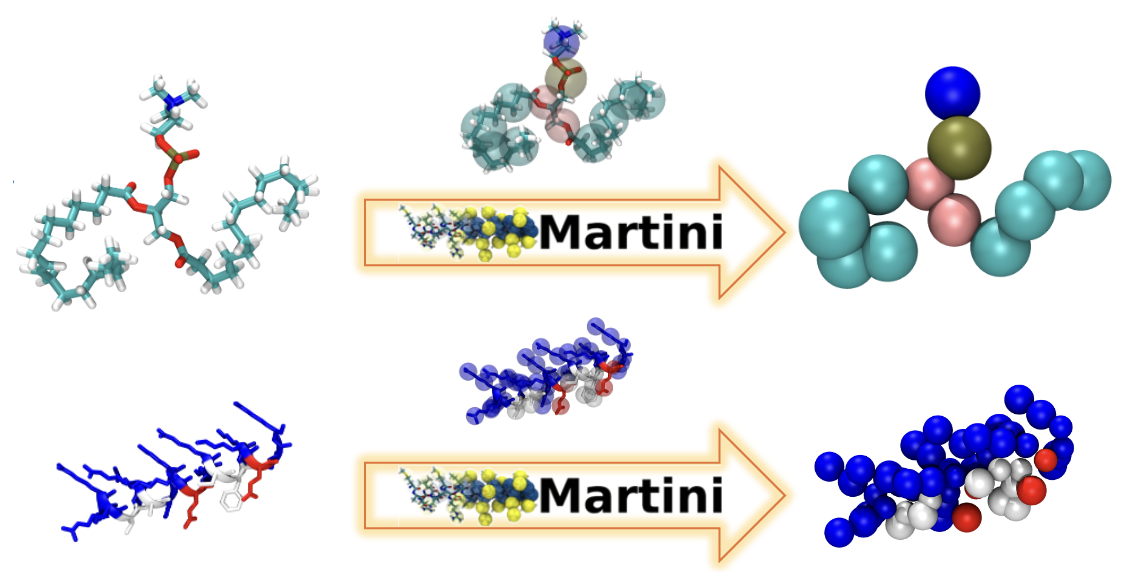
\includegraphics[width=0.99\linewidth]{General_Sections/Figures/AA2CG.png}
    \caption{Representation of the 3D structure of a lipid (up, POPC) and a peptide (bottom, KRRIRRAKKKEKRCFKKEKR) using an AA force field (left) and its corresponding mapping into Martini CG (right).}
    \label{fig:AA2CG}
\end{figure}

In the peptide--membrane simulations presented in the corresponding results chapter (see Section~\ref{art:metadynamics}), the Martini 2.2 coarse-grained force field~\cite{martini2} was employed to investigate the interaction and recognition mechanisms between AMPs and different biological membrane models. The use of a CG representation was motivated by the spatial and temporal scales associated with peptide--membrane recognition, which require extensive sampling and would therefore be computationally demanding with fully atomistic models. The reduced number of interaction sites and degrees of freedom substantially lowers the computational cost, making longer trajectories and larger membrane systems accessible.
The integration timestep in MD simulations is constrained by the fastest motions represented in the model, particularly high-frequency bond vibrations involving hydrogen atoms in atomistic descriptions~\cite{Feenstra1999}. Because these atomistic degrees of freedom are not explicitly represented in Martini, substantially larger integration timesteps can be used than in conventional AA-MD. For Martini 2.2, timesteps of 20--30~fs can be employed under appropriate simulation conditions, compared with the $\sim$2~fs commonly used in conventional AA-MD. This combination of reduced resolution and larger integration timesteps increases computational efficiency and facilitates simulations on the microsecond timescale.
Despite these advantages, conventional CG-MD may still be insufficient to efficiently sample rare peptide--membrane recognition events separated by free-energy barriers. To enhance sampling of these transitions, metadynamics was therefore combined with the CG-MD simulations. This approach promotes transitions between relevant conformational and configurational states and enables the reconstruction of the associated free-energy landscapes, providing a framework to characterize the energetics and specificity of peptide--membrane interactions.










\subsection{Metadynamics and free energy analysis}

\subsubsection{Standard metadynamics}

To understand the necessity of enhanced sampling methodologies, we must first establish the theoretical limitations of standard MD simulations. We consider a system governed by the conditions of the canonical ensemble. In this framework, the macroscopic state of the system is determined by the Helmholtz free energy, $A$, defined as:
\begin{equation}
    A = U - TS
\end{equation}
where $U$ is the internal energy, $T$ is the absolute temperature, and $S$ represents the entropy~\cite{termo_1,termo_2}. 

The mathematical justification for the approximation $\Delta A \approx \Delta G$ in condensed phases (liquids and solids) stems from the fundamental definitions of the relevant thermodynamic potentials. By definition, the Gibbs free energy ($G$) is expressed as:
\begin{equation}
    G = H - TS
\end{equation}
where $H$ is the enthalpy. The enthalpy itself is defined in terms of the internal energy, pressure ($P$), and volume ($V$) of the system:
\begin{equation}
    H = U + PV
\end{equation}

Substituting the definition of enthalpy into the equation for the Gibbs free energy yields:
\begin{equation}
    G = (U + PV) - TS = (U - TS) + PV
\end{equation}

Recognizing that the term $(U - TS)$ is precisely the definition of the Helmholtz free energy, we obtain the exact relationship between the two potentials:
\begin{equation}
    G = A + PV
\end{equation}

When analyzing a physical process or a transition between macroscopic states, the change in these thermodynamic potentials is denoted by the $\Delta$ operator:

\begin{equation}
    \Delta G = \Delta A + \Delta(PV)
\end{equation}

Applying the product rule, the expansion of the pressure-volume term gives $\Delta(PV) = P\Delta V + V\Delta P$. If the physical process occurs under typical experimental conditions at constant pressure (an isobaric process, where $\Delta P = 0$), the $V\Delta P$ term vanishes, and the equation simplifies to:
\begin{equation}
    \Delta G = \Delta A + P\Delta V
\end{equation}

For systems in condensed phases (liquids and solids), the materials are highly incompressible. Consequently, any volume change ($\Delta V$) during a chemical reaction, conformational transition, or thermal fluctuation is negligibly small ($\Delta V \approx 0$). Because the change in volume is minute, the mechanical work term $P\Delta V$ is physically insignificant compared to the characteristic magnitudes of the energetic and entropic contributions ($\Delta U$ and $T\Delta S$) involved in the process.

By neglecting the $P\Delta V$ term, we arrive at the condensed phase approximation~\cite{termo_1,termo_2}:
\begin{equation}
    \Delta G \approx \Delta A
\end{equation}

From a methodological standpoint, this derivation is crucial in computational physics and molecular simulation. It formally justifies why the results obtained from simulations in the canonical ensemble can be directly employed to study macroscopic processes that occur at constant pressure, which are governed by the Gibbs free energy~\cite{termo_1,termo_2}.

\paragraph{Equilibrium constants and ergodicity breaking}

When studying a system that transitions between two macroscopic states, $A$ and $B$, statistical mechanics dictates that the probability of observing the system in either state is proportional to its respective partition function~\cite{termo_1,termo_2}:
\begin{equation}
    P_A = \frac{Z_A}{Z}, \quad P_B = \frac{Z_B}{Z}
\end{equation}

The equilibrium constant, $K$, is defined as the ratio of these populations:
\begin{equation}
    K = \frac{P_B}{P_A} = \frac{Z_B}{Z_A}
\end{equation}

By relating the free energy of each state to its partition function ($A = -k_B T \ln Z$), the free energy difference between the two states, $\Delta A$, can be expressed entirely in terms of the equilibrium constant:
\begin{equation}
    \Delta A = A_B - A_A = -k_B T \ln Z_B + k_B T \ln Z_A = -k_B T \ln \frac{Z_B}{Z_A} = -k_B T \ln K
\end{equation}

This fundamental relationship demonstrates that $\Delta A$ fully determines the relative populations of the states and the equilibrium constant. Consequently, calculating the free energy surface (FES) along a chosen reaction coordinate, $\xi$, requires evaluating the marginal probability distribution, $P(\xi)$. This is achieved by integrating the Boltzmann factor over all degrees of freedom except $\xi$~\cite{termo_1,termo_2}:
\begin{equation}
    Z(\xi) = \frac{\int \delta[\xi'(r) - \xi] e^{-\beta E} d^N r}{\int e^{-\beta E} d^N r}
\end{equation}
where the denominator is the total partition function and the numerator evaluates the integral restricted to microstates where the system's coordinates $r$ correspond to the value $\xi$.

In a standard MD simulation, phase space is explored through a single, continuous time trajectory~\cite{termo_metad_presion,termo_1,termo_2}. Under the ergodic hypothesis, commonly assumed in statistical mechanics for systems at thermodynamic equilibrium, the ensemble average equates to the time average in the limit of infinite simulation time:
\begin{equation}
    Z(\xi) = P(\xi) = \lim_{t \to \infty} \frac{1}{t} \int_0^t \rho[\xi(t')] dt'
\end{equation}

However, the probability of visiting a specific configuration with energy $E$ is dictated by the Boltzmann distribution, $P(E) \propto \exp\left(-\frac{E}{k_B T}\right)$~\cite{termo_1,termo_2}. Because this probability is exponentially sensitive to energy, low-energy regions are sampled correctly, whereas high-energy transition states are rarely visited. When a system possesses high energy barriers ($\Delta A \gg k_B T$), the time required to spontaneously cross these barriers vastly exceeds feasible simulation lengths. Consequently, the assumption of infinite simulation time breaks down, ergodicity is broken, and the exact calculation of $\Delta A$ using standard MD becomes impossible.
Conventional MD simulations are often hindered by the timescale problem, trapping the system in local minima of the FES separated by high free-energy barriers~\cite{Laio2002}. To overcome this timescale bottleneck, various enhanced sampling methods have been proposed, such as Replica Exchange MD, Steered MD, and Umbrella Sampling. However, these methods may require extensive prior knowledge of the system, scale poorly with complex reaction coordinates, or lack adaptability~\cite{termo_metad_presion}.

This limitation motivated the development of history-dependent biasing methods, most notably metadynamics (MetaD)~\cite{termo_metad_presion}. Rather than waiting for the system to spontaneously cross high free-energy barriers, MetaD accelerates the exploration of the free-energy landscape by introducing a history-dependent bias potential along a set of predefined slow degrees of freedom, known as collective variables (CVs), denoted as $\vec{s}(\vec{q})$.

The basic idea is to progressively discourage the system from revisiting regions of CV space that have already been explored. This is achieved by depositing small repulsive Gaussian potentials along the trajectory at regular time intervals. As these Gaussians accumulate, previously visited free-energy minima are progressively filled, reducing the effective barriers and promoting transitions to less explored regions of the CV space. In this sense, MetaD can be viewed as a dynamical biasing scheme that progressively flattens the free-energy landscape along the selected CVs.

Instead of evolving solely under the original potential energy function $U(\vec{q})$, the system evolves under a time-dependent biased potential:
\begin{equation}
U_{\mathrm{bias}}(\vec{q},t)
=
U(\vec{q}) + V(\vec{s}(\vec{q}),t)
\end{equation}
where $V(\vec{s},t)$ is the history-dependent bias potential acting on the selected CVs~\cite{termo_metad_presion}.

The bias potential is constructed as a sum of Gaussian kernels periodically deposited along the trajectory in CV space:
\begin{equation}\label{eq:metad_bias}
V(\vec{s},t)
=
\sum_{k\tau < t}
W(k\tau)
\exp\left[
-\sum_{i=1}^{d}
\frac{
\left(s_i-s_i(\vec{q}(k\tau))\right)^2
}{2\sigma_i^2}
\right]
\end{equation}
where $\tau$ is the deposition stride, $W(k\tau)$ is the height of the Gaussian deposited at time $k\tau$, and $\sigma_i$ is its width along the $i$-th CV. Here, $\vec{q}(k\tau)$ denotes the microscopic coordinates of the system at the deposition time, such that $s_i(\vec{q}(k\tau))$ defines the center of the corresponding Gaussian in CV space.

The statistical-mechanical basis of MetaD follows from the relationship between the equilibrium probability distribution of the CVs, $P(\vec{s})$, and the corresponding free-energy surface:
\begin{equation}
F(\vec{s}) = -k_{\mathrm{B}}T\ln P(\vec{s}) + C
\end{equation}
where $C$ is an arbitrary additive constant. By continuously modifying the sampling distribution through the accumulated bias, MetaD reduces the probability of repeatedly visiting already sampled regions and promotes exploration of higher free-energy regions.

Under the assumption that the selected CVs provide a suitable description of the slow degrees of freedom and that the bias is deposited sufficiently slowly, the accumulated bias approaches the negative of the underlying free-energy surface in CV space. In the long-time limit,
\begin{equation}
V(\vec{s},t\rightarrow\infty)
\approx
-F(\vec{s}) + C
\end{equation}
Consequently, the biased free-energy landscape becomes approximately flat along the selected CVs, allowing the system to explore regions that would be rarely visited in an unbiased simulation. The accumulated bias can therefore be used to reconstruct the underlying free-energy surface and estimate the relative thermodynamic stability of the sampled states without requiring prior knowledge of the transition pathways~\cite{termo_metad_presion}.

\begin{figure}[!htbp]
    \centering
    \includesvg[width=0.65\linewidth]{General_Sections/Figures/metadynamics_comparison.svg}
    \caption{Progressive evolution of a one-dimensional model potential $V(s)$ by metadynamics bias. The thick black curve is the starting potential with two wells and a central barrier. Thin colored lines (from dark purple to yellow) represent the dynamic evolution of the sum of Gaussians along a trajectory that first explores the left well, then crosses the barrier, and finally visits the right well.}
    \label{fig:metad}
\end{figure}




\subsubsection{Well-Tempered metadynamics}

In standard metadynamics, Gaussian bias potentials of fixed height are continuously deposited along the selected collective variables (CVs), progressively discouraging the system from revisiting previously sampled regions of the CV space. This promotes the exploration of configurations separated by free-energy barriers. However, the continuous deposition of Gaussians can lead to persistent fluctuations in the accumulated bias and does not result in the same asymptotic behavior as Well-Tempered Metadynamics (WTMetaD).

WTMetaD introduces a bias-dependent scaling of the Gaussian height, such that the magnitude of newly deposited Gaussians decreases as the bias accumulates~\cite{Barducci2008}. The height of a Gaussian deposited at time $t=k\tau$ is given by:

\begin{equation}
W (k \tau ) = W_0 \exp \left( -\frac{V(\vec{s}(\vec{q}(k \tau)),k \tau)}{k_B\Delta T} \right )
\end{equation}

where $W_0$ is the initial Gaussian height, $V(\vec{s},t)$ is the accumulated bias potential, $k_B$ is the Boltzmann constant, and $\Delta T$ is a parameter controlling the rate at which the Gaussian height decreases.

The degree of tempering is commonly expressed through the bias factor $\gamma$,

\begin{equation}
\gamma
=
\frac{T+\Delta T}{T}
\end{equation}

The parameter $\Delta T$ does not represent an actual increase in the physical temperature of the system. Instead, it controls the extent to which the sampling distribution is broadened along the biased CVs. In the long-time limit, the WTMetaD bias converges, up to an additive constant, to a fraction of the underlying free-energy surface:

\begin{equation}
V(\vec{s},t\rightarrow \infty) = -\frac{\Delta T}{T+\Delta T}F(\vec{s}) + C = -\left(1 - \frac{1}{\gamma}\right)F(\vec{s}) + C
\end{equation}

where $F(\vec{s})$ is the free-energy surface and $C$ is an arbitrary constant. Thus, the bias factor determines the degree to which the free-energy landscape is compensated during the simulation. In the limit $\gamma\rightarrow1$, the biasing effect vanishes, whereas increasing $\gamma$ progressively approaches the behavior of standard MetaD~\cite{Barducci2008}.

\paragraph{Practical considerations and limitations}
Despite its theoretical guarantees, the performance of (WT)MetaD in practice depends critically on several methodological choices. First, the quality of the reconstructed free-energy surface is inherently limited by the choice of CVs: if the selected variables do not capture all relevant slow degrees of freedom, important free-energy barriers may remain unsampled and the resulting FES will be incomplete~\cite{Bussi2020}. Second, the deposition parameters (Gaussian height $W_0$, width $\sigma_i$, and stride $\tau$) must be chosen carefully. Excessively large or narrow Gaussians can lead to over-biasing or insufficient resolution of the free-energy surface, respectively. Third, although WTMetaD is guaranteed to converge to a well-defined stationary distribution, convergence can be slow for high-dimensional CV spaces or systems with multiple competing slow modes. In practice, convergence is assessed by monitoring the time evolution of the accumulated bias and verifying that free-energy profiles computed from successive portions of the trajectory become stationary~\cite{termo_metad_presion}.

\subsubsection{Thermodynamic reweighting}

Because the system evolves under a time-dependent bias, the configurations generated during a WTMetaD simulation are sampled from a distribution that differs from the unbiased canonical ensemble. Statistical reweighting can therefore be used to account for the effect of the applied bias when estimating thermodynamic observables.

If the biased Hamiltonian is written as:

\begin{equation}
H'(\vec{q},\vec{p},t)
=
H(\vec{q},\vec{p})
+
V(\vec{s}(\vec{q}),t)
\end{equation}

the corresponding statistical weight required to recover the unbiased distribution is related to the Boltzmann factor of the bias. For a given configuration, the reweighting factor can be expressed schematically as:

\begin{equation}
w(\vec{q},t)
\propto
\exp\left[
\frac{V(\vec{s}(\vec{q}),t)}
{k_B T}
\right]
\end{equation}

These weights allow observables to be estimated from the biased trajectory while accounting for the effect of the metadynamics potential. In particular, they can be used to reconstruct free-energy profiles along coordinates different from those directly biased during the simulation, provided that the relevant regions of configurational space have been sufficiently sampled. Reweighting does not compensate for insufficient sampling and therefore cannot recover information about configurations or regions of phase space that were not adequately explored.



\subsubsection{Selection and formulation of collective variables}

The success of an enhanced sampling calculation depends critically on the choice of collective variables (CVs). Ideally, the selected CVs should capture the slow or otherwise relevant degrees of freedom associated with the transitions between the metastable states of interest. An inappropriate choice of CVs may result in inefficient sampling or hinder the reconstruction of the underlying free-energy landscape~\cite{Bussi2020}. In the study of AMP--membrane interactions, CVs are commonly defined as geometric descriptors of the association and orientation of the peptide relative to the membrane. For example, peptide--membrane distance and orientational variables such as tilt or rotation angles can be used to characterize the main degrees of freedom involved in membrane recognition and insertion~\cite{DANI_METADINAMICA}.

\paragraph{Geometrical framework of the peptide--membrane system}

To define the CVs used to characterize peptide--membrane association, the system is described geometrically in a three-dimensional Cartesian coordinate system, with the $z$-axis defined as the normal to the membrane plane. The peptide and membrane are represented by their respective centers of mass (COM), together with vectors describing the orientation of the peptide relative to the membrane.

\textbf{Distance and insertion depth.} Let $\vec{R}_{\mathrm{mem}}$ and $\vec{R}_{\mathrm{pep}}$ denote the centers of mass of the membrane and peptide, respectively. For a set of particles with masses $m_i$ and positions $\vec{r}_i$, the center of mass is given by:

\begin{equation}
\vec{R}_{\mathrm{mem}} = \frac{1}{M_{\mathrm{mem}}} \sum_{i\in\mathrm{mem}} m_i\vec{r}_i,
\qquad
\vec{R}_{\mathrm{pep}} = \frac{1}{M_{\mathrm{pep}}} \sum_{j\in\mathrm{pep}} m_j\vec{r}_j
\end{equation}

where:

\begin{equation}
M_{\mathrm{mem}}=\sum_{i\in\mathrm{mem}}m_i,
\qquad
M_{\mathrm{pep}}=\sum_{j\in\mathrm{pep}}m_j
\end{equation}

are the corresponding total masses. The peptide--membrane separation vector is then defined as:

\begin{equation}
\vec{D} = \vec{R}_{\mathrm{pep}} - \vec{R}_{\mathrm{mem}}
\end{equation}

The component of this vector along the membrane normal,

\begin{equation}
D_z = \vec{D}\cdot\hat{z}
\end{equation}

provides a measure of the peptide's position along the membrane-normal direction and is therefore used as a CV for the translational component of membrane association. The corresponding Euclidean distance between the two centers of mass is:

\begin{equation}
D = ||\vec{D}|| = \sqrt{D_x^2+D_y^2+D_z^2}
\end{equation}

While $D$ describes the overall separation between the peptide and membrane COMs, $D_z$ specifically characterizes their relative displacement along the membrane normal. For a membrane lying approximately in the $xy$ plane, this coordinate provides a direct measure of the peptide's approach towards and displacement across the bilayer along the principal insertion direction.

\paragraph{Peptide orientation and tilt angle}

The orientation of the peptide relative to the membrane is characterized by an internal peptide axis defined from the centers of mass of the N- and C-terminal residues. Let $\vec{N}$ and $\vec{C}$ denote these positions,

\begin{equation}
\vec{N} = \vec{r}_{\mathrm{N-term}},
\qquad
\vec{C} = \vec{r}_{\mathrm{C-term}}
\end{equation}

The peptide axis is then defined as:

\begin{equation}
\vec{h} = \vec{C}-\vec{N},
\qquad
\hat{h} = \frac{\vec{h}}{||\vec{h}||}
\end{equation}

The \textbf{tilt angle} $\theta$ is defined as the angle between the peptide axis and the membrane normal $\hat{z}$:

\begin{equation}
\theta =
\arccos\left(\hat{h}\cdot\hat{z}\right)
\end{equation}

Thus, $\theta=0^\circ$ corresponds to an orientation in which the peptide axis is parallel to the membrane normal, whereas $\theta=90^\circ$ corresponds to an orientation in which the peptide axis lies parallel to the membrane plane. In this definition, $\theta$ characterizes the inclination of the peptide with respect to the membrane and therefore provides the principal rotational coordinate associated with its orientation.

\paragraph{Internal rotation around the peptide axis}

The tilt angle alone does not fully specify the orientation of an elongated peptide. In particular, two peptides with the same $\theta$ can differ in the orientation of their side-chain distribution around the longitudinal axis. To describe this degree of freedom, an internal rotation angle $\phi$ is introduced.

A molecular reference vector $\hat{\mu}$ is first defined from the peptide backbone and projected onto the plane perpendicular to the peptide axis,

\begin{equation}
\hat{\mu}_{\perp} = \frac{ \hat{\mu}-(\hat{\mu}\cdot\hat{h})\hat{h} }{ \left| \hat{\mu}-(\hat{\mu}\cdot\hat{h})\hat{h} \right| }
\end{equation}

A reference direction within the plane perpendicular to $\hat{h}$ is defined using the membrane normal, and a second orthogonal direction is obtained as (based on the definition by Esteban-Martín and Salgado~\cite{ESTEBANMARTIN20074278}):


\begin{equation}
\hat{t} = \hat{h}\times \frac{ \hat{z}\times\hat{h} }{ |\hat{z}\times\hat{h}| }
\end{equation}


The internal rotation angle can then be expressed using the two components of $\hat{\mu}_{\perp}$ in this local reference frame ((Figure \ref{fig:eulers_angles})):
 \begin{equation}
\phi = \mathrm{sgn}\left( \hat{h} \cdot (\hat{t} \times \hat{\mu}_\perp) \right) \cdot \arccos\left( \hat{\mu}_\perp \cdot \hat{t} \right)
\end{equation}
where the sign correction ensures a continuous mapping of the full $360^\circ$ rotation. Periodic boundary conditions are taken into account when constructing all position vectors involved in these calculations.

The reference frame becomes singular when $\hat{h}$ is parallel to $\hat{z}$, since $|\hat{z}\times\hat{b}|=0$. This corresponds to the limiting case $\theta=0^\circ$. In practice, configurations approaching this singularity are handled by imposing a minimum norm threshold when constructing the local frame.

\paragraph{Relevant orientational degrees of freedom}

The orientation of the peptide with respect to the membrane can be described by three rotational coordinates. The tilt angle $\theta$ specifies the inclination of the peptide axis relative to the membrane normal, while $\phi$ specifies the rotation of the molecular structure around that axis. A third angle would describe the azimuthal direction of the peptide axis within the membrane plane (Figure \ref{fig:eulers_angles}).

For the present system, this latter coordinate is not included as a collective variable because the membrane plane does not provide a fixed in-plane reference direction for the peptide. In particular, for a homogeneous and laterally isotropic membrane, a global rotation of the system within the membrane plane does not change the relative membrane--peptide configuration. The relevant orientational information can therefore be represented by the tilt and internal rotation angles.

Together with the translational coordinate $D_z$, the CV space used to characterize peptide--membrane association is therefore defined by (see Section \ref{art:metadynamics}):

\begin{equation}
\left(D_z,\theta,\phi\right)
\end{equation}

which captures the peptide displacement along the membrane normal, its inclination relative to the membrane, and its rotation around its longitudinal axis. These coordinates provide a reduced geometrical description of the principal translational and orientational changes involved in peptide association with the membrane.


\begin{figure}[!ht]
    \centering
    \includesvg[width=0.75\linewidth]{General_Sections/Figures/helix_geometry.svg}
    \caption{Definition of the generalized coordinates $q$ for a helical peptide in a 3-D coordinate system.
    The peptide (represented by the blue helix) is modeled as a rigid body whose configuration is fully described by a set of generalized coordinates $q \in \mathbb{R}^6$. This set comprises three translational degrees of freedom, $(x, y, z)$, and three rotational degrees of freedom, $(\psi, \theta, \phi)$, corresponding to the Euler angles. 
    The translation coordinates $(x, y)$ denote the position of the peptide within the membrane plane, while $z$ represents the insertion depth along the membrane normal. Regarding orientation, $\theta$ (tilt angle) defines the inclination relative to the $Z$-axis, $\psi$ (azimuthal angle) describes the orientation of the tilt in the $XY$ plane, and $\phi$ represents the internal rotation of the helix about its longitudinal axis $\mathbf{\hat{n}}$. 
    Assuming an infinite, homogeneous, and isotropic membrane in the $XY$ plane, the system exhibits translational symmetry along $X$ and $Y$, as well as rotational symmetry around the $Z$-axis. Consequently, the potential energy of the system is independent of $x, y$, and $\psi$ (ignorable coordinates), effectively reducing the configurational study to the three biologically relevant degrees of freedom: insertion depth ($z$), tilt ($\theta$), and internal rotation ($\phi$).}
    \label{fig:eulers_angles}
\end{figure}



\subsubsection{Dimensionality reduction of free energy surfaces}

A free-energy surface (FES) obtained from multiple collective variables can be projected onto a lower-dimensional space when only a subset of the variables is required for a particular analysis. Such a projection must account for the statistical weight associated with the degrees of freedom that are integrated out. Consequently, a thermodynamic projection cannot, in general, be obtained by taking a cross-section of the original FES or by selecting the minimum-energy value along the discarded coordinate.

For a two-dimensional FES $F(s_1,s_2)$, the corresponding equilibrium probability density in the collective-variable space is related to the free energy through the Boltzmann relation,

\begin{equation}
F(s_1,s_2) = -k_B T \ln P(s_1,s_2) + C
\end{equation}

where $k_B$ is the Boltzmann constant, $T$ is the temperature, and $C$ is an arbitrary additive constant. Equivalently,

\begin{equation}
P(s_1,s_2)
\propto
\exp\left[
-\frac{F(s_1,s_2)}{k_B T}
\right]
\end{equation}

The thermodynamic projection onto $s_1$ is obtained by marginalizing the probability density over the discarded variable $s_2$:

\begin{equation}
P(s_1) = \int P(s_1,s_2)\,ds_2
\end{equation}

Substituting the Boltzmann relation gives:

\begin{equation}
P(s_1)
\propto
\int
\exp\left[
-\frac{F(s_1,s_2)}{k_B T}
\right]
ds_2
\end{equation}

The corresponding one-dimensional free-energy profile is then obtained from the marginal probability,

\begin{equation}
F(s_1) = -k_B T\ln P(s_1)+C'
\end{equation}

or, equivalently,

\begin{equation}
F(s_1) = -k_B T \ln \left[ \int \exp\left( -\frac{F(s_1,s_2)}{k_B T} \right) ds_2 \right] +C''
\end{equation}

where $C''$ absorbs the normalization constants. This expression shows that the projected free energy accounts for the statistical contribution of all configurations along the discarded coordinate. In contrast, a minimum-energy projection would retain only the lowest value of $F(s_1,s_2)$ at each $s_1$ and therefore would not preserve the corresponding configurational entropy.

In practice, the resulting profile is defined up to an arbitrary additive constant. For visualization and comparison, it is therefore conventional to shift the profile such that its minimum is equal to zero.


\paragraph{Computational implementation}

In practice, thermodynamic projections of multidimensional free-energy surfaces can be obtained during post-processing using the \texttt{sum\_hills} utility of the PLUMED package. When a subset of the collective variables is specified using the \texttt{--idw} option, the remaining variables are integrated out in the reconstruction of the free-energy surface. The corresponding thermal energy, $k_B T$, must be provided through the \texttt{--kt} option in energy units consistent with those used for the bias potential~\cite{plumed}.

For example, a two-dimensional FES defined by $s_1$ and $s_2$ can be projected onto $s_1$ using

\begin{verbatim}
plumed sum_hills --hills HILLS --idw s1 --kt 2.5
\end{verbatim}

Here, \texttt{--idw s1} specifies $s_1$ as the variable retained in the projected FES, while the remaining CV, $s_2$, is integrated out. The \texttt{--kt} value specifies the thermal energy used in this integration. Consequently, the resulting one-dimensional profile corresponds to a thermodynamic marginalization over the discarded CV rather than to a simple minimum-energy projection~\cite{plumed}.




\subsubsection{Calculation of the standard binding free energy ($\Delta G^0$)}

The FES obtained from enhanced-sampling simulations provides a description of the relative stability of the peptide configurations sampled along the selected collective variables. To quantify the thermodynamic affinity of a peptide for a membrane and to facilitate comparison between different membrane models, a standard Gibbs free energy of binding, $\Delta G^0$, can be obtained by integrating the corresponding potential of mean force (PMF) and applying a standard-state correction~\cite{Woo2005}.

From statistical thermodynamics, the probability of observing a microscopic state with energy $W$ at temperature $T$ is proportional to its Boltzmann factor,

\begin{equation}
p \propto e^{-\beta W}
\end{equation}

where $\beta=(k_B T)^{-1}$, with $k_B$ denoting the Boltzmann constant. For a peptide interacting with a membrane, the configurational state can in general be described by its translational coordinates $\vec{r}$ and orientational degrees of freedom $\Upsilon$. The corresponding configurational partition function per unit volume can be expressed as:

\begin{equation}
\frac{q}{V}
=
\frac{1}{V}
\int
e^{-\beta W(\vec{r},\Upsilon)}
d\vec{r},d\Upsilon
\end{equation}

The partition coefficient $\kappa$ between the bound ($b$) and free ($f$) states is defined as the ratio of their probabilities per unit volume,

\begin{equation}
\kappa
=
\frac{p_b/V_b}{p_f/V_f}
=
\frac{q_b/V_b}{q_f/V_f}
\end{equation}

For the peptide--membrane system considered here, the PMF is projected onto the membrane-normal coordinate $z$, with the bulk region defined such that the peptide--membrane interaction is negligible beyond a distance $\lambda$. Under this one-dimensional approximation, the partition coefficient is obtained from the Boltzmann-weighted integral of the PMF,

\begin{equation}
\kappa
=
\frac{1}{\lambda}
\int_0^\lambda
e^{-\beta W(z)}
,dz
\end{equation}

where $\lambda$ defines the range of the membrane-associated region considered in the calculation. The corresponding free energy of association is:

\begin{equation}
\Delta G
=
-k_B T\ln(\kappa)
\end{equation}

To express this quantity relative to the conventional standard concentration of $1$ M, a standard-state correction is introduced. The volume corresponding to one molecule at a concentration of $1$ M is:

\begin{equation}
V_0
=
\frac{1}{C_0}
=
\frac{1~\mathrm{L}}{N_A}
\approx
1660~\text{\AA}^3
\end{equation}

where $C_0=1$ M and $N_A$ is Avogadro's constant. Because the PMF is expressed along a one-dimensional reaction coordinate, the corresponding standard-state length scale is given by $V_0^{1/3}$. Following the formulation used for peptide--membrane adsorption~\cite{DANI_CUANTICA}, the standard-state partition coefficient is therefore:

\begin{equation}
\kappa^0
=
\kappa
\frac{\lambda}{V_0^{1/3}}
=
\frac{1}{V_0^{1/3}}
\int_0^\lambda
e^{-\beta W(z)}
,dz
\end{equation}

The standard Gibbs free energy of binding is subsequently calculated as:

\begin{equation}
\Delta G^0
=
-k_B T\ln(\kappa^0)
\end{equation}

This formulation provides a standard-state free energy of peptide--membrane association based on the PMF along the membrane-normal coordinate. The resulting value depends on the definition of the bound and reference regions and on the one-dimensional approximation adopted for the calculation. Consequently, comparisons with experimental binding free energies should be interpreted within the same thermodynamic and state definitions.



















\section{Statistical methods and error analysis}

Molecular dynamics simulations generate trajectories consisting of a large number of configurations sampled over time. The analysis of these trajectories involves calculating averages, fluctuations, correlations, and other statistical quantities from the sampled data. Because consecutive configurations are generally correlated, the statistical information contained in a trajectory cannot be assessed solely from the total number of recorded frames. Appropriate statistical treatment is therefore required both to obtain representative estimates of the properties of interest and to quantify their associated uncertainties~\cite{tratamiento_datos_fisicos}.

In this work, statistical analysis is applied to the time series and structural data obtained from the molecular dynamics simulations. The methods described in this section include the calculation of temporal averages, the treatment of statistical uncertainty arising from autocorrelation through block averaging, and dimensionality-reduction and clustering techniques used to characterize the conformational space explored by the simulations. These approaches provide the basis for the quantitative analysis of the simulated systems and the identification of distinct conformational states.



\subsection{Sample and temporal averages}

For a set of $N$ discrete observations of a quantity $x$, the sample mean is defined as:
\begin{equation}
\langle x \rangle = \frac{1}{N}\sum_{n=1}^{N}x_n
\end{equation}
When the quantity is expressed as a function of time, $x(t)$, its temporal average over a time interval $T$ is given by:
\begin{equation}
\bar{x} =
\frac{1}{T}
\int_{t_0}^{t_0+T} x(t'),dt'
\end{equation}
In practice, MD trajectories provide discrete observations separated by a sampling interval $\Delta t$. The temporal average can therefore be approximated by the arithmetic mean of the sampled trajectory frames:
\begin{equation}
\bar{x}
\approx
\frac{1}{N}
\sum_{n=1}^{N}
x(t_0+n\Delta t)
\end{equation}
where $T=N\Delta t$. Here, $\Delta t$ denotes the interval between consecutive observations used for the analysis and does not necessarily correspond to the integration time step of the MD simulation. In particular, coordinates and other observables are typically saved less frequently than the integration step in order to limit data storage and avoid redundant sampling.


\subsection{The autocorrelation problem and block averaging}
Most of the analyses performed in this work generate time series of physical quantities. To extract statistically meaningful conclusions from these data, it is necessary to quantify the uncertainty associated with the calculated averages. Following the treatment by Gómez Rodríguez et al.~\cite{tratamiento_datos_fisicos}, for a set of $N$ observations, the dispersion of the data is characterized by the sample variance $s^2(x)$, estimated as:
\begin{equation}
s^2(x) =
\frac{1}{N-1}
\sum_{n=1}^{N}
\left(x_n-\langle x\rangle\right)^2
\label{eq:variance}
\end{equation}
where $\langle x\rangle$ is the sample mean. The corresponding sample standard deviation, $s(x)=\sqrt{s^2(x)}$, characterizes the fluctuations of individual observations around the mean.
For error estimation, however, it is necessary to distinguish $s(x)$ from the standard deviation of the mean, or standard error, denoted as $\sigma_{\langle x\rangle}$. This quantity represents the uncertainty associated with the estimated average. If the $N$ observations were statistically independent and uncorrelated, the standard error would be given by:
\begin{equation}
\sigma_{\langle x\rangle}
=
\frac{s(x)}{\sqrt{N}}
\label{eq:std_error}
\end{equation}

A fundamental challenge in molecular dynamics simulations is that consecutive observations in a trajectory are generally not statistically independent, but instead exhibit temporal correlations. Consequently, the assumption underlying equation~\ref{eq:std_error} is not valid for correlated trajectories. Using the total number of frames $N$ in this case leads to an underestimation of the statistical uncertainty, because the effective number of independent observations is smaller than the total number of recorded frames.
To account for these correlations, the Block Averaging method was employed following the procedure introduced by Flyvbjerg and Petersen~\cite{block_average}. The original data set of $N$ observations is divided into $N'=N/k$ consecutive blocks of size $k$. The mean of each block $i$ is calculated as:
\begin{equation}
M_i =
\frac{1}{k}
\sum_{j=1}^{k}
x_{(i-1)k+j}
\end{equation}
The resulting block averages constitute a new statistical sample with a reduced number of observations. As the block size $k$ is progressively increased, correlations between neighboring block averages are reduced. The statistical error of the mean is evaluated as a function of the block size, and a plateau in the estimated error indicates convergence of the statistical uncertainty, suggesting that the remaining correlations between blocks are negligible.
Following the blocking analysis, the final uncertainty $\sigma$ and its associated statistical uncertainty $\sigma_{\sigma}$ are estimated as:
\begin{equation}
\sigma
\approx
\sqrt{\frac{s^2(M)}{N'-1}},
\qquad
\sigma_{\sigma}
\approx
\frac{\sigma}{\sqrt{2(N'-1)}}
\end{equation}
where $s^2(M)$ denotes the variance of the set of block averages and $N'$ is the number of blocks at the selected block size. The second expression provides an estimate of the statistical uncertainty associated with the calculated error itself.
This procedure accounts for the temporal correlations present in MD trajectories and therefore provides a more reliable estimate of the uncertainty associated with trajectory-derived quantities than the assumption of statistically independent observations. It was consequently used to estimate the statistical uncertainties reported for the free-energy surfaces and other quantities derived from the simulations.




\subsection{Principal component analysis}
Principal Component Analysis (PCA) is a fundamental statistical method in multivariate analysis that performs a linear transformation of the coordinate system. From a mathematical perspective, PCA is a change of basis that maps the data from its original high-dimensional space to a new orthogonal coordinate system whose axes are ordered according to the amount of variance they capture.
Let us consider a data set consisting of $n$ observations and $d$ variables, represented by a data matrix $\mathbf{X} \in \mathbb{R}^{n \times d}$. To ensure that the covariance matrix describes the fluctuations around the mean, the data are first centered such that each variable has zero mean:
\begin{equation}
[\mathbf{X}]_{ij} \leftarrow [\mathbf{X}]_{ij} - \bar{x}_j
\end{equation}
where $\bar{x}_j$ is the mean of the $j$-th variable. The covariance between these variables is then described by the covariance matrix $\mathbf{C} \in \mathbb{R}^{d \times d}$, defined as:
\begin{equation}
\mathbf{C} = \frac{1}{n-1} \mathbf{X}^T \mathbf{X} =
\begin{pmatrix}
\mathrm{Var}(x_1) & \mathrm{Cov}(x_1,x_2) & \cdots & \mathrm{Cov}(x_1,x_d) \\
\mathrm{Cov}(x_2,x_1) & \mathrm{Var}(x_2) & \cdots & \mathrm{Cov}(x_2,x_d) \\
\vdots & \vdots & \ddots & \vdots \\
\mathrm{Cov}(x_d,x_1) & \mathrm{Cov}(x_d,x_2) & \cdots & \mathrm{Var}(x_d)
\end{pmatrix}
\end{equation}
The diagonal elements represent the variance of each individual variable, whereas the off-diagonal elements represent the covariance between pairs of variables. Non-zero covariance values indicate that fluctuations in different variables are statistically related and therefore contain overlapping information.
The core objective of PCA is to identify a new set of orthogonal axes, known as principal directions, along which the variance of the data is maximized and the projected variables are mutually uncorrelated. These directions are obtained by diagonalizing the covariance matrix through an eigenvalue decomposition:
\begin{equation}
\mathbf{C}\mathbf{V} = \mathbf{V}\mathbf{\Lambda}
\end{equation}
where $\mathbf{V}$ is an orthogonal matrix whose columns are the eigenvectors $\vec{v}_i$, and $\mathbf{\Lambda}$ is a diagonal matrix containing the corresponding eigenvalues $\lambda_i$. The eigenvectors define the directions of the principal axes, while the corresponding eigenvalues quantify the variance of the data along those directions.
The original data can then be projected onto the principal directions according to:
\begin{equation}
\mathbf{Y} = \mathbf{X}\mathbf{V}
\end{equation}
The columns of $\mathbf{Y}$ are the principal component scores, representing the coordinates of the observations in the new basis. Because the covariance matrix is diagonal in this basis, these projected variables are mutually uncorrelated. The eigenvectors are conventionally ordered according to decreasing eigenvalue,
\begin{equation}
\lambda_1 \geq \lambda_2 \geq \dots \geq \lambda_d
\end{equation}
so that the first principal components account for the largest fractions of the total variance. Consequently, the dimensionality of the data can be reduced by retaining only the first few components, thereby obtaining a lower-dimensional representation while preserving as much of the original variance as possible.

\subsection{K-means clustering}
To further characterize the conformational states of a molecular system and identify representative structures, clustering methods such as K-means can be applied to molecular dynamics trajectories. K-means is an unsupervised learning algorithm that partitions a set of observations into $K$ distinct clusters according to their proximity in the selected feature space~\cite{MacQueen1967,Lloyd1982}. In MD analysis, the observations may correspond to trajectory frames represented by Cartesian coordinates, principal component scores, or other collective variables.
The K-means algorithm iteratively minimizes the within-cluster sum of squares (WCSS), also referred to as inertia. Given an initial set of $K$ centroids, each observation is represented by a feature vector $\vec{x}_i$ and assigned to the cluster with the nearest centroid $\vec{\mu}_j$. The centroids are then recalculated as the mean of the feature vectors assigned to each cluster, and the procedure is repeated until the cluster assignments or centroids converge. The objective function can be written as:

\begin{equation}
    \min_{\{S_j\}_{j=1}^{K}}
    \sum_{j=1}^{K}
    \sum_{\vec{x}_i \in S_j}
    \left\|
    \vec{x}_i-\vec{\mu}_j
    \right\|^2
\end{equation}

where $S_j$ denotes the $j$-th cluster. The objective is therefore to minimize the sum of squared Euclidean distances between each observation and the centroid of its assigned cluster.




























































%%%%%%% CONTINUAR
\section{Quantum computing}
A central computational challenge in the study and design of antimicrobial peptides is the enormous size of the sequence and conformational spaces that must be considered. For a peptide of length \(L\), the number of possible sequences composed of the 20 standard amino acids grows exponentially as \(20^L\), making exhaustive enumeration impractical even for relatively short peptides~\cite{Levinthal_paradox,robert2021resource}. Moreover, each sequence can adopt multiple three-dimensional conformations, whose relative stability and accessibility depend on the molecular environment. This dependence is particularly relevant for membrane-active peptides, for which the conformational ensemble can change substantially upon interaction with lipid interfaces~\cite{paper_paula,vogel_amps}.

The difficulty of exploring such conformational spaces is commonly illustrated by the Levinthal paradox~\cite{Levinthal_paradox,Levinthal_paradox_2}. An exhaustive and unbiased sampling of all possible conformations would require an astronomically large number of configurations, incompatible with the timescales observed for protein and peptide folding. The resolution of this apparent paradox is that molecular folding does not proceed through a random enumeration of all possible conformations. Instead, the physical interactions between residues constrain the accessible conformational pathways and give rise to a highly non-uniform energy landscape~\cite{Levinthal_paradox,robert2021resource,Levinthal_paradox_2}. Nevertheless, identifying the relevant low-energy states and characterizing the transitions between them remains computationally challenging, particularly when several slow degrees of freedom and environmental interactions contribute to the dynamics.


\subsection{Computational challenges and the NISQ era}
The computational complexity of biomolecular optimization can also be considered from the perspective of formal complexity theory. Protein folding and related structure-prediction problems have been shown to be computationally difficult under several simplified formulations, including lattice models and contact-map representations~\cite{robert2021resource}. These results should not be interpreted as a direct proof that continuous molecular dynamics is NP-hard. Rather, they illustrate the combinatorial nature of simplified formulations of the underlying optimization problem. In practical molecular simulations, the main difficulty arises from the combination of a large configuration space, complex energy landscapes, and the computational cost required to sample them adequately.
Machine-learning (ML) methods provide an alternative strategy by learning relationships between sequence, structure, and experimentally or computationally derived properties. AlphaFold, for example, demonstrated that deep-learning models can predict protein structures with high accuracy for many classes of proteins~\cite{Jumper2021}. Such approaches, however, primarily target structure prediction rather than explicit simulation of the physical pathways connecting conformational states. Consequently, they do not directly provide molecular free-energy landscapes or dynamical trajectories, and their treatment of environment-dependent interactions depends on the information represented in the model and its training data. These considerations are particularly relevant for peptide--membrane systems, where lipid composition, interfacial environment, and conformational transitions can play a central role~\cite{PROTEINMPNN,ROSETTA,Goverde2024,dolorfino2024,platform_ia_2,ia_lim_big}.
ML-based approaches have also been applied to the exploration and optimization of peptide sequence space. For example, ApexGO combines generative modelling with Bayesian optimization to identify peptide sequences with predicted improvements in antimicrobial activity~\cite{Torres2026}. In this framework, sequence optimization is driven by a learned predictor of minimum inhibitory concentration rather than by an explicit physical energy function. Consequently, the optimization is constrained by the properties represented in the predictor and by the distribution of sequences and experimental conditions available to the underlying model~\cite{Torres2026}. This illustrates a general distinction between data-driven and physics-based approaches: ML methods can efficiently navigate large sequence spaces, whereas their predictions and optimization objectives remain dependent on the scope and assumptions of the learned models.
Physics-based approaches, such as MD, explicitly evaluate molecular interactions according to a predefined molecular-mechanics force field and provide access to conformational dynamics and, with appropriate sampling methods, to thermodynamic quantities. Their applicability is nevertheless constrained by the computational cost of evaluating the potential energy and by the difficulty of sampling processes separated by high free-energy barriers or involving slow collective variables. These limitations become particularly relevant for peptide--membrane recognition, where association, reorientation, insertion, and conformational changes may occur on different timescales~\cite{computational_expensive_MD}. Thus, MD and ML provide complementary approaches: ML can efficiently explore large data-defined spaces, whereas physics-based simulations provide an explicit model of the interactions governing the sampled molecular dynamics.
These complementary limitations motivate the investigation of alternative computational formulations in which selected molecular problems can be expressed as energy-based optimization problems. QC provides a framework for representing and manipulating such optimization problems using quantum states and quantum operations. In an $N$-qubit system, the state is represented in a $2^N$-dimensional Hilbert space~\cite{nielsen2010quantum,robert2021resource}. This exponential state-space dimension, however, does not imply that all $2^N$ amplitudes can be directly accessed or that every problem formulated on a quantum computer obtains a computational advantage. Any potential advantage depends on the specific encoding, quantum algorithm, cost function, and measurement strategy~\cite{nielsen2010quantum,preskill1998quantum}.
The present work is situated within the Noisy Intermediate-Scale Quantum (NISQ) era, in which quantum processors operate with limited numbers of noisy qubits and without the full fault-tolerant error correction required for large-scale quantum algorithms~\cite{preskill1998quantum}. Practical performance is therefore affected by hardware noise, qubit connectivity, gate fidelity, circuit depth, coherence times, and the number of measurements required to estimate the relevant observables~\cite{Shor1995,KITAEV20032}. Accordingly, the objective of the quantum-computing component of this work is not to establish quantum advantage, but to investigate how selected peptide-related problems can be formulated as quantum optimization problems and to assess the associated computational requirements and limitations under currently available hardware and simulation conditions.


\subsection{Foundations of quantum information}
To understand the application of quantum algorithms to molecular design, it is useful to first introduce the basic units of quantum information and the mathematical operations used to manipulate them. Quantum information theory provides a framework for encoding and processing information according to the principles of quantum mechanics, using quantum states and operations that differ fundamentally from their classical counterparts~\cite{nielsen2010quantum,preskill1998quantum}.
\subsubsection{Qubits and multi-qubit systems}
The fundamental unit of quantum information is the quantum bit, or \textit{qubit}. Analogously to a classical bit, a qubit has two orthogonal computational basis states, conventionally denoted by $|0\rangle$ and $|1\rangle$. Physically, these two states can be encoded in different quantum systems, such as two energy levels of an atom, the internal states of an ion, or the states of a superconducting circuit~\cite{nielsen2010quantum,preskill1998quantum}.
Qubits are mathematically represented using Dirac's \textit{ket} notation. A common representation of the computational basis states is given by the column vectors:
\begin{equation}
|0\rangle =
\begin{pmatrix}
1\\
0
\end{pmatrix},
\qquad
|1\rangle =
\begin{pmatrix}
0\\
1
\end{pmatrix}
\end{equation}
Unlike a classical bit, whose state is restricted to either $0$ or $1$, a qubit can be described as a coherent linear combination of the two computational basis states. A general pure qubit state is therefore written as:
\begin{equation}
|\psi\rangle = \alpha|0\rangle + \beta|1\rangle =
\begin{pmatrix}
\alpha\\
\beta
\end{pmatrix}
\end{equation}
where $\alpha,\beta\in\mathbb{C}$ are complex probability amplitudes. The state must satisfy the normalization condition:
\begin{equation}
|\alpha|^2+|\beta|^2=1
\end{equation}
such that $|\alpha|^2$ and $|\beta|^2$ correspond to the probabilities of obtaining the respective computational basis states upon measurement.
The state space of multiple qubits is constructed through the tensor product of the individual qubit Hilbert spaces. For a system of $N$ qubits, the corresponding Hilbert space is:
\begin{equation}
\mathcal{H}_N=(\mathbb{C}^2)^{\otimes N}
\end{equation}
which has dimension $2^N$. Its computational basis consists of all binary strings of length $N$, denoted by $z\in\{0,1\}^N$. Consequently, a general pure state of the system can be expressed as:
\begin{equation}
|\psi\rangle =
\sum_{z\in\{0,1\}^N}
\alpha_z |z\rangle,
\qquad
\text{with}
\qquad
\sum_{z\in\{0,1\}^N}|\alpha_z|^2=1
\end{equation}
where each $\alpha_z\in\mathbb{C}$ is the probability amplitude associated with the computational basis state $|z\rangle$. The normalization condition ensures that the probabilities of all possible measurement outcomes sum to unity~\cite{nielsen2010quantum,preskill1998quantum}.
A single-qubit pure state can also be represented geometrically on the surface of the unit sphere, known as the Bloch sphere (see Figure~\ref{fig:bloch_sphere}). Up to an overall global phase, any pure qubit state can be parameterized by two angles, $\theta$ and $\phi$, as:
\begin{equation}
|\psi\rangle =
\cos\left(\frac{\theta}{2}\right)|0\rangle
+
e^{i\phi}
\sin\left(\frac{\theta}{2}\right)|1\rangle,
\qquad
0\leq\theta\leq\pi,
\qquad
0\leq\phi<2\pi
\end{equation}
The corresponding Bloch vector is:
\begin{equation}
\vec{r}=
\left(
\sin\theta\cos\phi,
\sin\theta\sin\phi,
\cos\theta
\right)
\end{equation}
where $\theta$ determines the polar angle with respect to the $Z$ axis and $\phi$ determines the azimuthal angle in the $XY$ plane. The computational basis states $|0\rangle$ and $|1\rangle$ correspond to the north and south poles of the sphere, respectively, as illustrated in Figure~\ref{fig:bloch_sphere}.

\begin{figure}[!htbp]
    \centering
    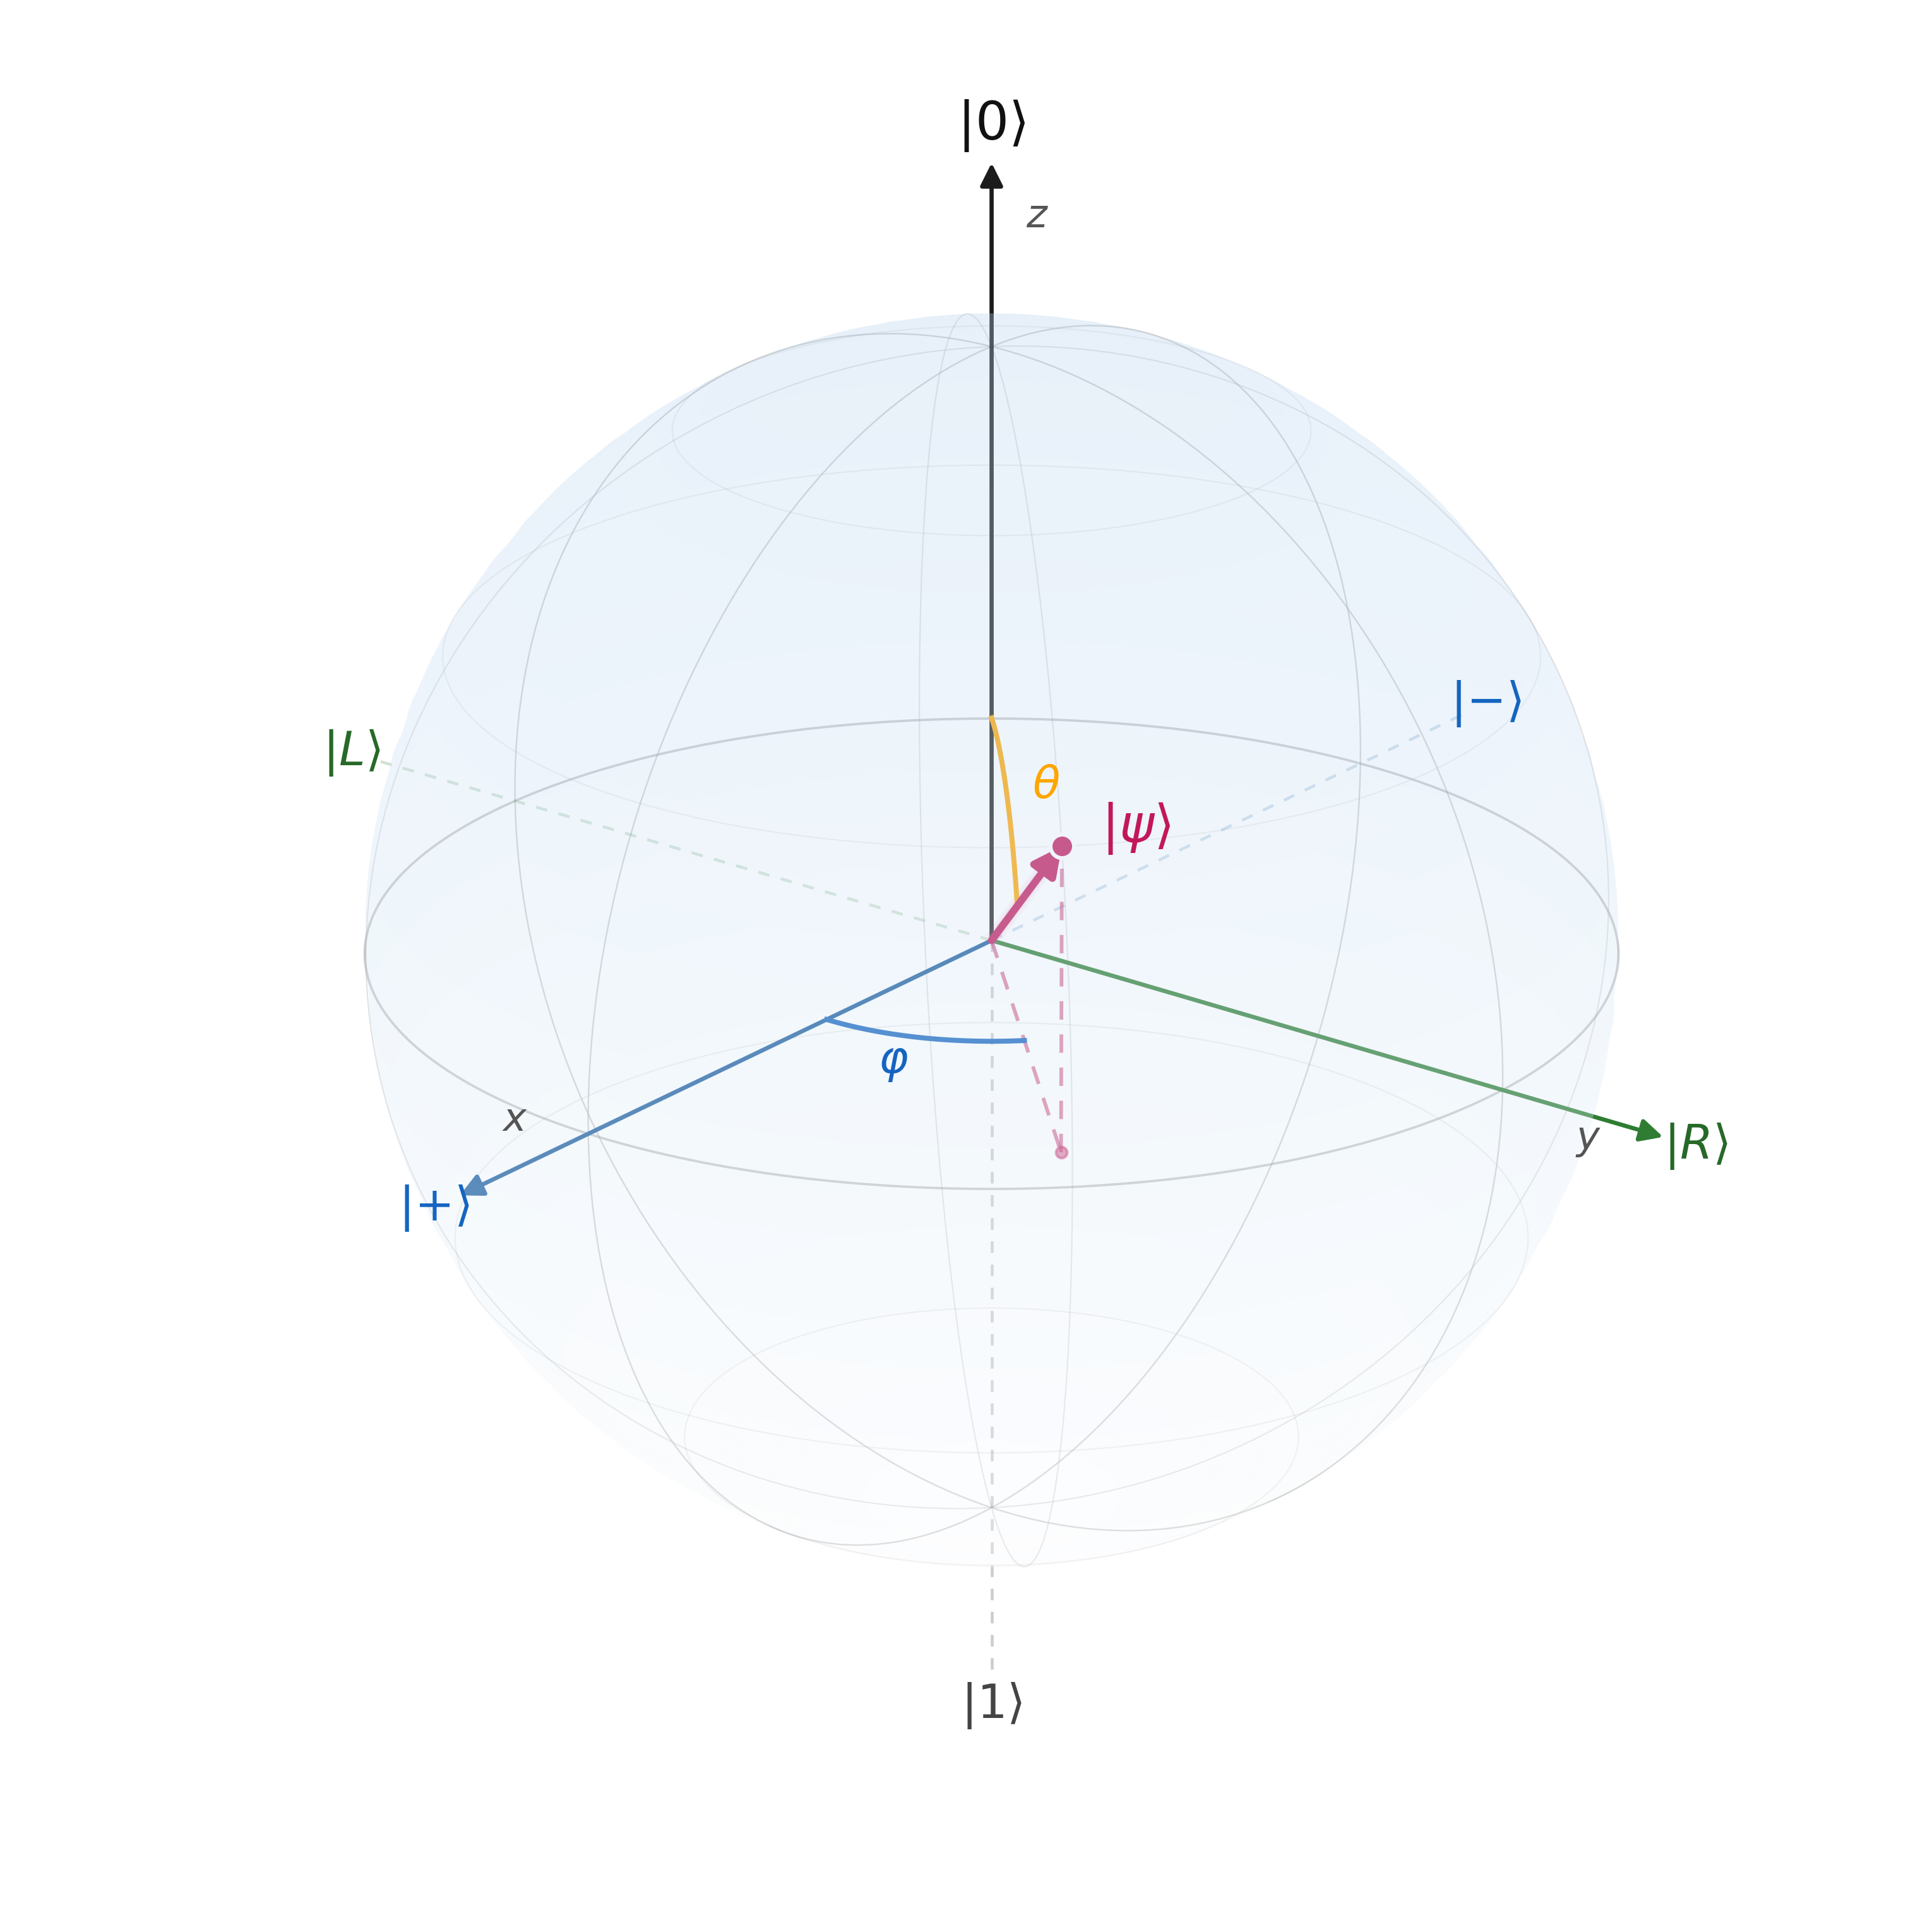
\includegraphics[width=0.6\linewidth]{General_Sections/Figures/esfera_bloch_tesis.png}
    \caption{The Bloch sphere representation of a single-qubit state. The angles $\theta$ and $\phi$ determine the position of the state vector on the surface of the sphere. The $Z$-axis corresponds to the computational basis states $|0\rangle$ and $|1\rangle$, while the $X$ and $Y$ axes describe the relative coherence and phase between their probability amplitudes.}
    \label{fig:bloch_sphere}
\end{figure}

\subsubsection{Unitary dynamics and quantum gates}
Analogous to classical computers, which employ elementary logic gates such as AND or NOT to perform deterministic operations on bits, quantum computers use quantum gates to manipulate the states and probability amplitudes of one or more qubits. The continuous-time evolution of a closed quantum system is governed by the time-dependent Schr\"odinger equation (adopting natural units such that $\hbar=1$)~\cite{nielsen2010quantum}:
\begin{equation}
i\frac{d|\psi(t)\rangle}{dt}=\hat{H}|\psi(t)\rangle
\end{equation}
The Hamiltonian operator $\hat{H}$ is the observable associated with the total energy of the quantum system. Its eigenstates $|\psi_i\rangle$ and corresponding eigenvalues $E_i$ satisfy:
\begin{equation}
\hat{H}|\psi_i\rangle=E_i|\psi_i\rangle
\end{equation}
For an $N$-qubit system, $\hat{H}$ is a $2^N\times2^N$ Hermitian operator. Its eigenstates form an orthonormal basis of the Hilbert space, in which the Hamiltonian admits the spectral decomposition:
\begin{equation}
\hat{H}=\sum_{i=1}^{2^N}E_i|\psi_i\rangle\langle\psi_i|
\end{equation}
When the Hamiltonian is time-independent, the formal solution of the Schr"odinger equation can be expressed through the unitary time-evolution operator:
\begin{equation}
\hat{U}(t)=e^{-i\hat{H}t}
\end{equation}
such that an initial state $|\psi(0)\rangle$ evolves according to:
\begin{equation}
|\psi(t)\rangle=\hat{U}(t)|\psi(0)\rangle
\end{equation}
Because $\hat{U}(t)$ is unitary, it preserves inner products and, consequently, the normalization of the quantum state. In gate-based quantum computing, general unitary transformations are implemented through sequences of discrete quantum gates. These gates therefore provide the elementary operations used to construct quantum circuits and approximate or synthesize the desired unitary evolution.

\paragraph{Pauli and rotation gates}
The Pauli operators constitute a fundamental set of single-qubit operators and form the basis for many quantum operations and Hamiltonian representations. They are both Hermitian and unitary:
\begin{equation}
\sigma_x \equiv X = \begin{pmatrix} 0 & 1 \\ 1 & 0 \end{pmatrix}, \quad 
\sigma_y \equiv Y = \begin{pmatrix} 0 & -i \\ i & 0 \end{pmatrix}, \quad 
\sigma_z \equiv Z = \begin{pmatrix} 1 & 0 \\ 0 & -1 \end{pmatrix}
\end{equation}
The Pauli-$X$ operator acts as a bit-flip, analogous to the classical NOT operation, mapping:
\begin{equation}
X|0\rangle=|1\rangle,
\qquad
X|1\rangle=|0\rangle
\end{equation}
The Pauli-$Z$ operator leaves $|0\rangle$ unchanged while introducing a relative phase of $\pi$ to $|1\rangle$:
\begin{equation}
Z|0\rangle=|0\rangle,
\qquad
Z|1\rangle=-|1\rangle
\end{equation}
Another fundamental single-qubit gate is the Hadamard gate, $H$, which transforms computational basis states into equal superpositions:
\begin{equation}
H=\frac{1}{\sqrt{2}}
\begin{pmatrix}
1&1\\
1&-1
\end{pmatrix}
\end{equation}
with:
\begin{equation}
H|0\rangle=|+\rangle=
\frac{|0\rangle+|1\rangle}{\sqrt{2}},
\qquad
H|1\rangle=|-\rangle=
\frac{|0\rangle-|1\rangle}{\sqrt{2}}
\end{equation}
These states lie on the equator of the Bloch sphere and constitute the eigenstates of the Pauli-$X$ operator.
Parameterized rotation gates provide continuous control over the state of a qubit and are particularly important in variational quantum algorithms. They are defined as:
\begin{equation}
R_x(\theta)=e^{-i\theta X/2},
\qquad
R_y(\theta)=e^{-i\theta Y/2},
\qquad
R_z(\theta)=e^{-i\theta Z/2}
\end{equation}
For example, the $R_z$ gate introduces a relative phase between the computational basis states:
\begin{equation}
R_z(\theta)=
\begin{pmatrix}
e^{-i\theta/2}&0\\
0&e^{i\theta/2}
\end{pmatrix}
\end{equation}
\paragraph{Two-qubit gates and entanglement}
Single-qubit gates alone cannot generate entanglement from an initially separable state. Two-qubit gates, in contrast, can create correlations that cannot be represented as a product of independent single-qubit states. A fundamental example is the controlled-NOT (CNOT) gate, which flips a target qubit $q_t$ if and only if the control qubit $q_c$ is in the state $|1\rangle$:
\begin{equation}
CNOT=
\begin{pmatrix}
1&0&0&0\\
0&1&0&0\\
0&0&0&1\\
0&0&1&0
\end{pmatrix}
\end{equation}
For example, applying a CNOT gate to the separable state $|+\rangle\otimes|0\rangle$ produces the Bell state:
\begin{equation}
|+\rangle|0\rangle
\xrightarrow{CNOT}
\frac{|00\rangle+|11\rangle}{\sqrt{2}}
\end{equation}
which is an entangled state. This illustrates how two-qubit gates provide the mechanism for introducing entanglement into quantum circuits, a resource that plays a central role in many quantum algorithms.

\subsubsection{Measurement and hardware architectures}
Unlike classical readout, quantum measurement in the computational basis is a non-unitary and probabilistic process that projects the quantum state onto one of the computational basis states~\cite{nielsen2010quantum,preskill1998quantum}. For a state:
\begin{equation}
|\psi\rangle=\sum_z\alpha_z|z\rangle
\end{equation}
a measurement in the computational basis returns a particular classical bitstring $z$ with probability $|\alpha_z|^2$.
Because a measurement produces a single probabilistic outcome, the quantum state must generally be prepared repeatedly to characterize its underlying probability distribution. Repeated measurements, commonly referred to as \textit{shots}, yield a histogram of bitstrings from which measurement probabilities can be estimated. These probabilities should be distinguished from expectation values of observables. For an observable $\hat{O}$, its expectation value is estimated from the measurement outcomes as:
\begin{equation}
\langle\hat{O}\rangle
\approx
\frac{1}{N_{\mathrm{shots}}}
\sum_{k=1}^{N_{\mathrm{shots}}}o_k
\end{equation}
where $o_k$ denotes the measurement outcome associated with the $k$-th shot. The statistical standard error of this estimator is:
\begin{equation}
\sqrt{\frac{\mathrm{Var}(\hat{O})}{N_{\mathrm{shots}}}}
\end{equation}
showing that the statistical uncertainty decreases as $1/\sqrt{N_{\mathrm{shots}}}$~\cite{mcclean2016theory}. Thus, increasing the number of measurements improves the statistical precision, but does not by itself eliminate systematic errors arising from state-preparation, gate, or measurement imperfections.
For a Hamiltonian expressed as a weighted sum of measurable operators,
\begin{equation}
\hat{H}=\sum_j c_j\hat{P}_j
\end{equation}
where $\hat{P}_j$ are typically tensor products of Pauli operators, its expectation value can be reconstructed from the individual expectation values,
\begin{equation}
\sum_j c_j\langle\hat{P}_j\rangle
\end{equation}
This decomposition is particularly important for variational quantum algorithms, in which the expectation value of the Hamiltonian is repeatedly estimated from finite sets of measurements.
\paragraph{Hardware platforms}
Several physical architectures have been developed to implement qubits, each with different trade-offs in coherence, gate speed, connectivity, scalability, and experimental complexity.
\begin{itemize}
\item \textbf{Trapped-ion architecture:} Individual ions are confined in vacuum using electromagnetic fields, typically in radio-frequency Paul traps. Qubits are encoded in internal electronic or hyperfine states, while quantum gates are implemented using laser or microwave interactions. The shared vibrational modes of the ions can mediate high-fidelity entangling operations and provide long-range connectivity within an ion chain~\cite{trapped_ions}.

\item \textbf{Superconducting qubits:} These qubits are implemented using cryogenic superconducting circuits containing Josephson junctions. They offer fast gate operations and can be fabricated using established micro- and nanofabrication techniques, making them attractive for large-scale integration. Their main challenges include relatively short coherence times compared with some other platforms, control errors, crosstalk, and the requirement for sophisticated cryogenic infrastructure~\cite{superconductiong_qubits}.

\item \textbf{Photonic quantum computing:} Quantum information is encoded in properties of photons such as polarization, path, or temporal modes. Photonic systems offer low sensitivity to thermal environments and can operate without cryogenic cooling for many components. However, photon loss, efficient state generation and detection, and the implementation of deterministic two-photon interactions remain important experimental challenges. Entangling operations can therefore rely on measurement-based approaches, interference, or specialized nonlinear optical components~\cite{photonic_qubits}.
\end{itemize}



\subsection{Variational Quantum Algorithms}
Variational quantum algorithms (VQAs) constitute a class of hybrid quantum--classical algorithms designed to operate on near-term quantum hardware. Rather than relying exclusively on long, fully quantum circuits, VQAs distribute the computational workload between a Quantum Processing Unit (QPU) and a classical processor. The quantum processor prepares parameterized quantum states and evaluates the corresponding objective function through measurements, while a classical optimizer updates the circuit parameters based on the measured results~\cite{preskill1998quantum}. This iterative structure allows variational algorithms to operate with circuit depths compatible with current quantum hardware, although their performance remains constrained by hardware noise, circuit depth, measurement overhead, and the efficiency of the classical optimization procedure.
The implementation of VQAs is facilitated by software frameworks that provide tools for quantum-circuit construction, simulation, compilation, execution, and classical optimization. In this research, two complementary frameworks were primarily employed:
\begin{itemize}
\item \textbf{Qiskit}~\cite{Qiskit}: an open-source quantum computing framework developed by IBM that provides tools for constructing, simulating, transpiling, and executing quantum circuits on simulators and IBM quantum hardware.
\item \textbf{PennyLane}~\cite{pennylane}: a cross-platform framework for differentiable quantum programming that integrates quantum circuits with classical computational workflows. Its automatic-differentiation capabilities facilitate the optimization of parameterized quantum circuits using gradient-based and other classical optimization methods.
\end{itemize}
Within this thesis, two VQA-based approaches are considered for distinct optimization problems. The Variational Quantum Eigensolver (VQE) is employed to investigate peptide conformational optimization by encoding the corresponding energy function into a qubit Hamiltonian and minimizing its expectation value~\cite{DANI_CUANTICA}. The Quantum Approximate Optimization Algorithm (QAOA), in contrast, is employed to address discrete amino-acid sequence optimization under environment-dependent objectives~\cite{DANI_HAMILTONIAN}. Thus, VQE is used here to address an energy-minimization problem over a parameterized quantum state, whereas QAOA is used to explore a discrete combinatorial optimization landscape. The formulation, encoding strategy, ansatz, optimization procedure, and computational backend used for each problem are described separately in the corresponding results chapters (see Section~\ref{art:vqe_cesga} and \ref{art:hamiltonian}).



\subsubsection{Hamiltonians and parameterized circuits}
To formulate a physical or mathematical optimization problem on a quantum computer, its objective function must be encoded in terms of operators acting on a register of qubits. In the context of VQAs, this is commonly achieved by expressing the Hamiltonian $\hat{H}$ as a linear combination of tensor products of single-qubit Pauli operators.
The Pauli operators $X$, $Y$, and $Z$, together with the identity operator $I$, form a basis for the real vector space of Hermitian $2\times2$ operators. Consequently, any Hermitian operator acting on an $n$-qubit register can be expressed as a linear combination of tensor products of these single-qubit operators. The resulting set of $4^n$ Pauli strings forms a basis for the space of Hermitian operators acting on the $n$-qubit Hilbert space:
\begin{equation}
\hat{H} = \sum_i w_i P_i,
\qquad
P_i\in\{I,X,Y,Z\}^{\otimes n}
\end{equation}
where $w_i\in\mathbb{R}$ are the corresponding coefficients. This decomposition is central to VQAs because the expectation value of each Pauli string can be estimated experimentally through measurements in an appropriate basis, allowing the expectation value of the full Hamiltonian to be reconstructed from a finite set of measurable quantities.
The structure of the Hamiltonian depends on the optimization problem being considered. In VQE, $\hat{H}$ represents a physical or effective energy operator whose ground-state energy is sought and may contain non-commuting Pauli terms. According to the variational principle, the expectation value of the Hamiltonian for any normalized trial state provides an upper bound to the ground-state energy. In QAOA, the objective function is encoded in a cost Hamiltonian $\hat{H}_C$, which is typically diagonal in the computational basis and can therefore be expressed using products of $Z$ operators. The QAOA circuit additionally employs a mixer Hamiltonian, $\hat{H}_M$, which introduces transitions between computational-basis states.
The quantum state explored during a VQA is generated by a parameterized unitary circuit, commonly referred to as an \textit{ansatz}. Formally, the trial state is written as:
\begin{equation}
|\psi(\boldsymbol{\theta})\rangle = U(\boldsymbol{\theta})|0\rangle^{\otimes n}
\end{equation}
where $\boldsymbol{\theta}$ denotes the set of classical variational parameters. A commonly used circuit architecture is a layered ansatz,
\begin{equation}
U(\boldsymbol{\theta}) = \prod_{l=1}^{L}U_l(\boldsymbol{\theta}_l)
\end{equation}
where each layer may contain parameterized single-qubit rotations and entangling operations. The choice of ansatz determines the variational manifold accessible to the circuit and therefore represents an important compromise between expressibility, number of parameters, circuit depth, and susceptibility to optimization and hardware-related limitations~\cite{nielsen2010quantum}.
For a Hamiltonian decomposed into Pauli strings, the VQA objective function is given by:
\begin{equation}
C(\boldsymbol{\theta}) = \sum_i w_i
\langle\psi(\boldsymbol{\theta})|
P_i
|\psi(\boldsymbol{\theta})\rangle
\end{equation}
For VQE, minimizing this expectation value with respect to the variational parameters yields an approximation to the ground-state energy:
\begin{equation}
E_0
\leq
\min_{\boldsymbol{\theta}}
C(\boldsymbol{\theta})
\end{equation}
where $E_0$ denotes the exact ground-state energy. In practice, the individual expectation values $\langle P_i\rangle$ are estimated from repeated measurements of the quantum circuit. These measurements are combined according to the coefficients $w_i$ to evaluate the objective function, which is subsequently optimized by a classical optimization procedure.



\subsubsection{The Variational Quantum Eigensolver}
The Variational Quantum Eigensolver (VQE) is a hybrid quantum--classical algorithm designed to approximate the ground-state energy of a Hamiltonian~\cite{vqe_mejor}. Its theoretical basis is the Rayleigh--Ritz variational principle, which states that, for any normalized trial state $|\psi(\boldsymbol{\theta})\rangle$,
\begin{equation}
E(\boldsymbol{\theta}) = \langle\psi(\boldsymbol{\theta})|
\hat{H}
|\psi(\boldsymbol{\theta})\rangle
\geq E_0
\end{equation}
where $E_0$ is the ground-state energy of $\hat{H}$. VQE therefore seeks the set of variational parameters $\boldsymbol{\theta}$ that minimizes the expectation value,
\begin{equation}
E_0
\leq
\min_{\boldsymbol{\theta}}
E(\boldsymbol{\theta})
\end{equation}
If the chosen ansatz is sufficiently expressive to represent the ground state, the minimum of the variational energy approaches $E_0$ and, in the ideal case, reaches it. In practical implementations, however, the quality of the result depends on the expressibility and depth of the ansatz, the classical optimization procedure, statistical measurement uncertainty, and hardware noise.
\paragraph{Hardware-efficient and heuristic ansätze}
For near-term quantum hardware, hardware-efficient ansätze are commonly employed to balance variational flexibility against circuit depth and the number of quantum operations. These circuits typically combine parameterized single-qubit rotations with entangling gates, with their structure adapted to the connectivity and gate set of the target hardware. Examples available in Qiskit include \textit{RealAmplitudes} and \textit{EfficientSU2}~\cite{Qiskit}.
In this work, the \textit{RealAmplitudes} ansatz was employed for the VQE calculations. This parameterized circuit is constructed primarily from $R_y$ rotations and entangling gates and, under its standard construction, generates states with real amplitudes in the computational basis. Its relatively simple structure provides a suitable compromise between variational flexibility and circuit complexity for the conformational optimization problem considered in this work.
The choice of ansatz introduces a trade-off between expressibility and computational cost. Increasing the number of layers can enlarge the set of states that can be represented, but also increases circuit depth, parameter count, and susceptibility to hardware noise and optimization difficulties. Conversely, an overly restrictive ansatz may prevent the variational optimization from reaching states with sufficiently low energy.
\paragraph{The hybrid optimization loop}
The execution of VQE follows an iterative feedback loop between the quantum processor and a classical optimizer:
\begin{enumerate}
\item \textbf{State preparation (QPU):} The parameterized circuit $U(\boldsymbol{\theta})$ is applied to the initial state $|0\rangle^{\otimes n}$ to prepare the trial state $|\psi(\boldsymbol{\theta})\rangle$.
\item \textbf{Measurement (QPU):} The Pauli terms required to evaluate the Hamiltonian are measured repeatedly over a finite number of shots to estimate their expectation values.
\item \textbf{Cost evaluation (classical):} The measured expectation values are combined with the coefficients $w_i$ to calculate the variational energy,
\begin{equation}
C(\boldsymbol{\theta}) = \sum_i w_i
\langle P_i\rangle_{\boldsymbol{\theta}}
\end{equation}
\item \textbf{Parameter update (classical):} A classical optimization algorithm uses the evaluated objective to determine a new parameter vector $\boldsymbol{\theta}'$. Depending on the optimization strategy, this may involve gradient-free methods such as the Constrained Optimization BY Linear Approximations (COBYLA)~\cite{COBYLA} or the Simultaneous Perturbation Stochastic Approximation (SPSA)~\cite{SPSA}, or population-based methods such as differential evolution.
\item \textbf{Iteration:} The updated parameters are returned to the quantum processor, and the procedure is repeated until the selected convergence criterion is satisfied.
\end{enumerate}
The VQE procedure can therefore be viewed as an iterative optimization in which the quantum processor evaluates the energy associated with the current trial state, while the classical optimizer searches for the parameter vector that minimizes this energy. In the ideal case, convergence to the global minimum yields the ground-state energy of the Hamiltonian, provided that the chosen ansatz is capable of representing the corresponding ground state.




\begin{figure}[!htbp]
    \centering
    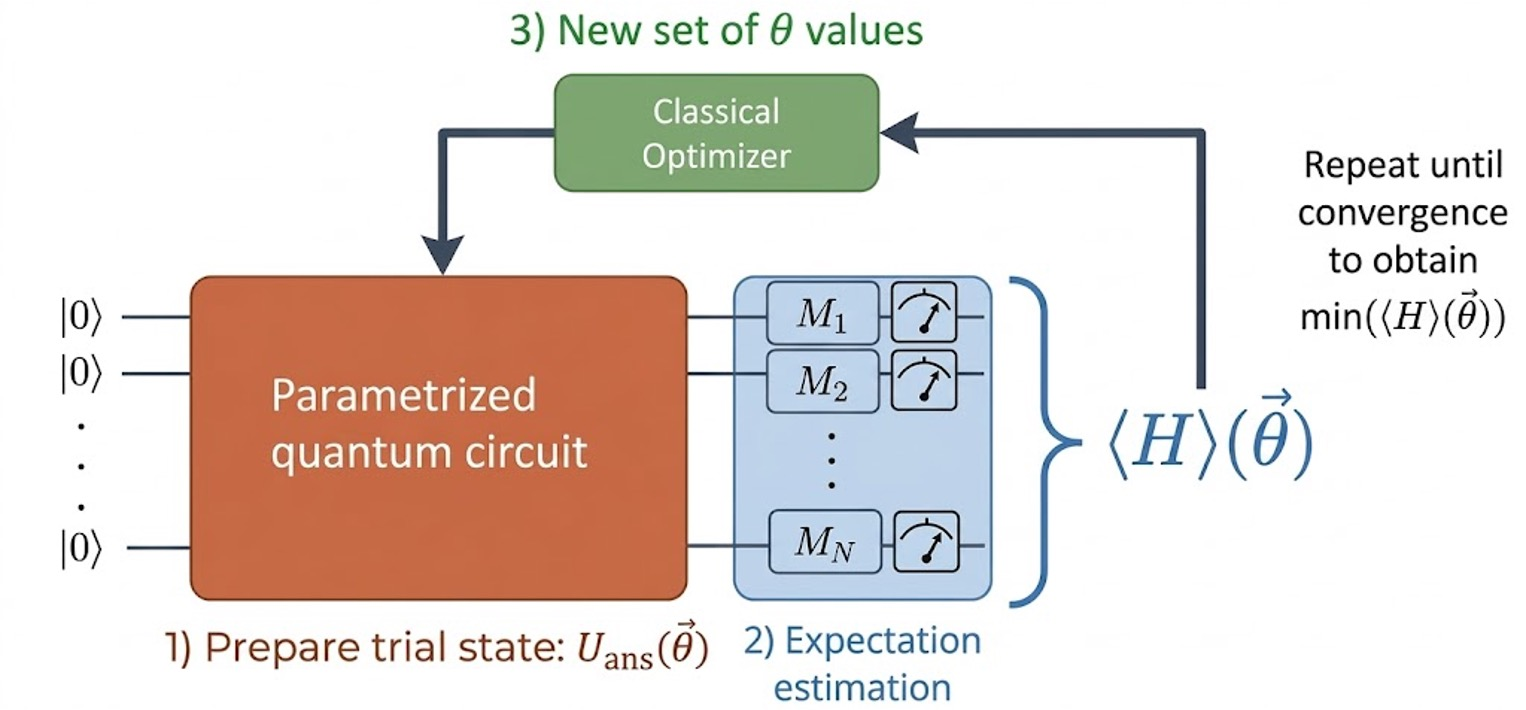
\includegraphics[width=0.8\linewidth]{General_Sections/Figures/vqe_demonstration.jpg}
    \caption{Schematic representation of the VQE hybrid architecture. The process illustrates the iterative feedback loop between the QPU, responsible for state preparation and measurement, and the CPU, which executes the optimization algorithm to update the variational parameters $\boldsymbol{\theta}$.}
    \label{fig:VQE_loop}
\end{figure}

\subsection{Combinatorial optimization on quantum devices}
While variational methods such as VQE are naturally formulated as energy-minimization problems over quantum states, many problems in computational biology involve discrete decision variables. Sequence design is one such example: at each position, a finite set of amino-acid identities must be selected, resulting in a combinatorial search space whose size grows exponentially with peptide length. Quantum optimization algorithms can address such problems by encoding the discrete variables into qubits and expressing the corresponding objective function as a cost Hamiltonian.
\subsubsection{Quadratic Unconstrained Binary Optimization (QUBO)}
The sequence-design problems considered in this research are formulated as Quadratic Unconstrained Binary Optimization (QUBO) problems~\cite{qubo_2}. A QUBO consists of minimizing a quadratic function of binary variables $x_i\in\{0,1\}$:
\begin{equation}
\min_{\mathbf{x}\in\{0,1\}^n} \quad \sum_i c_i x_i
+
\sum_{i<j}Q_{ij}x_ix_j
\end{equation}
where $c_i$ are the linear coefficients and $Q_{ij}$ describe pairwise interactions between binary variables. In the context of sequence design, these coefficients can encode contributions associated with individual amino-acid choices and pairwise interactions between selected residues.
QUBO formulations can be mapped to Ising Hamiltonians by introducing a binary-to-spin transformation. Using:
\begin{equation}
x_i=\frac{1-Z_i}{2}
\end{equation}
where $Z_i$ denotes the Pauli-$Z$ operator acting on qubit $i$, the QUBO objective can be transformed into a diagonal Hamiltonian of the form:
\begin{equation}
\hat{H}_C = K
+
\sum_i h_i Z_i
+
\sum_{i<j}J_{ij}Z_iZ_j
\end{equation}
where $K$, $h_i$, and $J_{ij}$ are the coefficients resulting from the binary-to-spin transformation. Because this Hamiltonian is diagonal in the computational basis, each binary configuration $\mathbf{x}$ corresponds to a computational-basis state $|\mathbf{x}\rangle$, and the corresponding eigenvalue reproduces the value of the original QUBO objective up to an additive constant. Since this constant does not affect the location of the minimum, the minimum-energy computational-basis state represents the optimal solution of the corresponding QUBO problem~\cite{qubo_1}.


\paragraph{Handling constraints via penalty terms}
Biological sequence-design problems are often subject to constraints, for example requiring a fixed number of selected residues, limiting the number of mutations, or enforcing a prescribed net charge. In a QUBO formulation, such constraints can be incorporated into the objective through penalty terms. For a set of linear constraints of the form:
\begin{equation}
A\mathbf{x}=\mathbf{b}
\end{equation}
a corresponding penalized objective can be written as:
\begin{equation}
f_{\mathrm{penalized}}(\mathbf{x}) = f(\mathbf{x})
+
\lambda
\left\|
A\mathbf{x}-\mathbf{b}
\right\|_2^2
\end{equation}
where $\lambda>0$ controls the energetic cost associated with constraint violations~\cite{qubo_2}. For binary variables, the identity $x_i^2=x_i$ ensures that expanding the quadratic penalty does not introduce terms of order higher than two. The resulting objective therefore remains within the QUBO form. The penalty coefficient must be chosen sufficiently large to discourage invalid configurations without unnecessarily dominating the original optimization objective.




\subsubsection{The Quantum Approximate Optimization Algorithm}
Once a discrete optimization problem has been expressed as a cost Hamiltonian $\hat{H}_C$, the QAOA can be used to search for low-energy computational-basis states. QAOA was introduced by Farhi, Goldstone, and Gutmann as a variational quantum algorithm for approximate combinatorial optimization~\cite{QAOA}. It constructs a parameterized quantum state by alternating the action of a cost Hamiltonian and a mixing Hamiltonian. The corresponding variational parameters are optimized classically using measurements obtained from the quantum circuit.
\paragraph{Connection with adiabatic quantum optimization}
The construction of QAOA is closely related to the principles of adiabatic quantum optimization. In the adiabatic approach, a quantum system is initialized in the ground state of an easily prepared Hamiltonian $\hat{H}_B$ and subsequently evolved according to a time-dependent Hamiltonian,
\begin{equation}
\hat{H}(t) = [1-s(t)]\hat{H}_B
+
s(t)\hat{H}_C
\end{equation}
where the schedule $s(t)$ varies continuously from $s(0)=0$ to $s(T)=1$. A commonly used initial or driver Hamiltonian is:
\begin{equation}
\hat{H}_M = -\sum_{i=1}^{N}X_i
\end{equation}
where $X_i$ denotes the Pauli-$X$ operator acting on qubit $i$. Its ground state is the uniform superposition:
\begin{equation}
|+\rangle^{\otimes N} = \left(\frac{|0\rangle+|1\rangle}{\sqrt{2}}\right)^{\otimes N}
\end{equation}
The cost Hamiltonian $\hat{H}_C$ encodes the classical optimization problem. Under ideal adiabatic evolution, the system remains close to the instantaneous ground state if the evolution is sufficiently slow relative to the relevant spectral gap and the rate at which the Hamiltonian changes~\cite{nielsen2010quantum}. The computational resources required to satisfy this condition depend strongly on the minimum spectral gap encountered along the chosen evolution path. For difficult optimization problems, this gap can become very small, potentially leading to evolution times that are impractical for near-term devices.
QAOA can be viewed as a variational, gate-based formulation motivated by this continuous evolution. Instead of following a prescribed continuous schedule, the evolution is replaced by an alternating sequence of cost and mixing unitaries. For a circuit with $p$ layers, the QAOA unitary can be written as:
\begin{equation}
\hat{U}(\boldsymbol{\gamma},\boldsymbol{\beta}) = \prod_{k=1}^{p}
e^{-i\beta_k\hat{H}_M}
e^{-i\gamma_k\hat{H}_C}
\end{equation}
where $\hat{H}_M$ denotes the mixing Hamiltonian, $\boldsymbol{\gamma}=(\gamma_1,\ldots,\gamma_p)$ and $\boldsymbol{\beta}=(\beta_1,\ldots,\beta_p)$ are independent sets of variational parameters, and $p$ determines the number of alternating layers. For the standard mixer $\hat{H}_M=-\sum_iX_i$, the initial state is chosen as the ground state of $\hat{H}_M$:
\begin{equation}
|\psi_p(\boldsymbol{\gamma},\boldsymbol{\beta})\rangle = \hat{U}(\boldsymbol{\gamma},\boldsymbol{\beta})
|+\rangle^{\otimes N}
\end{equation}
The connection with adiabatic evolution can be motivated by a Trotter-like discretization of the continuous evolution. However, QAOA is not simply a finite-step approximation of a fixed adiabatic schedule. The parameters $\boldsymbol{\gamma}$ and $\boldsymbol{\beta}$ are treated as free variational parameters and are optimized directly for the problem at hand. Increasing $p$ enlarges the variational flexibility of the circuit, but also increases its depth, number of operations, and susceptibility to hardware noise.
The QAOA objective function is given by the expectation value of the cost Hamiltonian,
\begin{equation}
F_p(\boldsymbol{\gamma},\boldsymbol{\beta}) = \langle
\psi_p(\boldsymbol{\gamma},\boldsymbol{\beta})
|
\hat{H}_C
|
\psi_p(\boldsymbol{\gamma},\boldsymbol{\beta})
\rangle
\end{equation}
The parameters are optimized iteratively using a classical optimizer. At each iteration, the QPU prepares the QAOA state and performs the measurements required to estimate the expectation value of the cost Hamiltonian. The classical optimizer then uses the resulting estimate of $F_p$ to determine updated values of $\boldsymbol{\gamma}$ and $\boldsymbol{\beta}$. At finite circuit depth, the variational optimization is not guaranteed to recover the global optimum, and the final result depends on the circuit depth, parameter initialization, optimization strategy, measurement uncertainty, and hardware noise.
A standard benchmark for QAOA is the MaxCut problem, which admits a direct mapping to an Ising cost Hamiltonian~\cite{max_cut_np_hard}. In this thesis, QAOA is instead applied to a peptide sequence-design problem, in which binary variables encode discrete amino-acid choices and the cost Hamiltonian represents an environment-dependent objective. This formulation allows the quantum circuit to act as a heuristic search procedure over a discrete sequence space while retaining an explicit energy-based representation of the optimization objective.


\begin{figure}[!htbp]
    \centering
    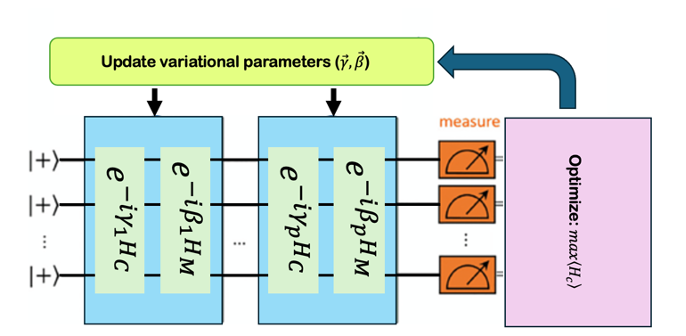
\includegraphics[width=0.8\linewidth]{General_Sections/Figures/qaoa_demonstration.png}
    \caption{Schematic representation of the QAOA circuit architecture for a depth $p$. The circuit begins with a layer of Hadamard gates to create a uniform superposition $|+\rangle^{\otimes N}$, followed by alternating layers of the cost unitary $e^{-i\gamma_k \hat{H}_C}$ and the mixer unitary $e^{-i\beta_k \hat{H}_B}$. Finally, the state is measured in the computational basis.}
    \label{fig:QAOA_circ}
\end{figure}

\paragraph{Conditional Value at Risk (CVaR) optimization}
In addition to the standard expectation-value objective, the QAOA optimization considered in this work employs the CVaR as an alternative objective function~\cite{cvar_1}. Whereas the expectation value incorporates all possible measurement outcomes according to their sampling probabilities, CVaR focuses specifically on the lower-energy tail of the sampled distribution. This provides a mechanism for directing the classical optimization towards regions of the parameter space that yield a higher probability of observing low-energy solutions.
For a confidence level $\alpha\in(0,1]$ and a fixed measurement budget of $K$ shots, let the measured energies be sorted in ascending order,
\begin{equation}
e_1 \leq e_2 \leq \dots \leq e_K
\end{equation}
The empirical CVaR estimator used in this work is defined as the mean energy of the lowest-energy fraction of the measured outcomes:
\begin{equation}
\mathrm{CVaR}_{\alpha} = \frac{1}{\lceil\alpha K\rceil}
\sum_{k=1}^{\lceil\alpha K\rceil} e_k
\end{equation}
Here, $\alpha=1$ corresponds to the mean energy over all measured outcomes, recovering the standard sample-mean objective. In contrast, smaller values of $\alpha$ progressively restrict the estimator to the lowest-energy outcomes. For example, $\alpha=0.1$ considers the lowest-energy $10\%$ of the measured samples. In the limit of small $\alpha$, the objective increasingly emphasizes the best observed outcomes, although it remains an estimator based on a finite number of measurements and therefore does not necessarily identify the true global optimum.
In this work, CVaR is used as an alternative objective function for the classical optimization of the QAOA parameters, rather than as a modification of the underlying quantum circuit. The QAOA state preparation and measurement procedure therefore remain unchanged; only the way in which the measured computational-basis outcomes are aggregated into the classical objective is modified.
The choice of $\alpha$ introduces a trade-off between the statistical information retained from the measurement distribution and the emphasis placed on low-energy outcomes. Decreasing $\alpha$ increases the focus on the lower-energy tail but reduces the number of samples contributing to the estimator, potentially increasing its statistical uncertainty for a fixed shot budget. Consequently, very small values of $\alpha$ may make the optimization more sensitive to sampling fluctuations. CVaR does not, by itself, eliminate hardware noise or measurement errors. Comparisons between CVaR and expectation-value optimization should therefore be performed using the same measurement budget and otherwise equivalent experimental conditions~\cite{cvar_1,cvar_2}.

\subsection{Classical optimization in hybrid workflows}
Variational quantum algorithms rely on a classical optimization procedure to update the parameters of the quantum circuit. The resulting objective landscape can be non-convex, while finite-shot measurements introduce statistical fluctuations and hardware noise can further perturb the objective evaluations. The choice of classical optimizer therefore constitutes an additional component of the computational workflow.
In this work, several derivative-free optimization approaches were explored during the development of the variational workflows. These methods do not require explicit gradient evaluation and can operate directly on objective functions affected by finite-shot sampling and hardware noise. Among the approaches considered were COBYLA, which provides a local model-based optimization strategy, and Differential Evolution (DE), a population-based stochastic optimization method~\cite{Failde2023,Kandala2017,DE,DE_2}.



\subsubsection{Constrained Optimization BY Linear Approximations}
Constrained Optimization BY Linear Approximations is a derivative-free, model-based optimization algorithm originally developed by M.~J.~D.~Powell for nonlinear constrained optimization~\cite{COBYLA}. At each iteration, COBYLA constructs local linear approximations of the objective function and constraints using function evaluations at a set of nearby points. These approximations are then optimized within a local region around the current solution.
For an $n$-dimensional parameter vector $\vec{x}$, the local subproblem can be expressed schematically as:
\begin{equation}
\begin{aligned}
\min_{\vec{x}\in\mathbb{R}^n}
\quad &
\hat{f}_k(\vec{x}) \\
\text{s.t.}\quad &
\hat{c}_{k,i}(\vec{x})\leq 0,
\quad i\in I,\\
&
\|\vec{x}-\vec{x}_k\|\leq\Delta_k,
\end{aligned}
\end{equation}
where $\hat{f}_k$ and $\hat{c}_{k,i}$ denote local linear approximations of the objective and constraint functions, respectively, $\vec{x}_k$ is the current iterate, and $\Delta_k$ defines the size of the local optimization region. Restricting the optimization to this region limits the step to a domain in which the linear approximations are expected to provide a useful description of the objective and constraints. The size of this region is subsequently adjusted according to the progress of the optimization.
For the variational circuits considered in this work, the optimization variables $\vec{x}$ correspond to the circuit parameters, such as rotation angles. Since COBYLA does not require analytical or quantum-measured gradients, it can be applied directly to objective functions obtained from finite-shot quantum measurements. This makes it suitable for hybrid quantum--classical workflows in which objective evaluations may be noisy or computationally expensive.
\subsubsection{Differential Evolution}
DE is a stochastic, population-based optimization algorithm introduced by Storn and Price for the global optimization of continuous parameter spaces~\cite{DE,DE_2}. Unlike local model-based methods, DE maintains a population of candidate solutions and generates new candidates using scaled differences between population members. This population-based strategy can promote exploration of different regions of a multimodal objective landscape without requiring gradient information.
At generation $g$, the population consists of $NP$ parameter vectors $\vec{x}_{i,g}$. The evolutionary process is based on three main operations:
\begin{itemize}
\item \textbf{Mutation:} A mutant vector is generated from a base population vector and a scaled difference between two other population members. For the commonly used DE/rand/1 strategy,
\begin{equation}
\vec{v}_{i,g} = \vec{x}_{r_1,g} + F\left(\vec{x}_{r_2,g} - \vec{x}_{r_3,g}\right)
\end{equation}
where $r_1$, $r_2$, and $r_3$ are distinct randomly selected indices and $F$ is the differential-weight parameter.
\item \textbf{Crossover:} The mutant vector is combined with the target vector $\vec{x}_{i,g}$ to generate a trial vector $\vec{u}_{i,g}$. For binomial crossover, each component is selected from the mutant vector with probability $C_r$, while the remaining components are inherited from the target vector. At least one component is typically forced to originate from the mutant vector to ensure that the trial vector differs from the target vector.
\item \textbf{Selection:} The trial vector is compared with its corresponding target vector according to the objective function. For a minimization problem, the candidate yielding the lower objective value is retained for the next generation.
\end{itemize}
The population-based nature of DE allows multiple candidate solutions to be explored simultaneously and does not rely on local gradient information. However, DE remains a stochastic heuristic and does not guarantee convergence to the global optimum. Its behavior can depend on factors including the population size, mutation strategy, crossover probability, parameter bounds, and the statistical noise associated with the objective-function evaluations.










\subsection{Challenges and noise mitigation in the NISQ era}
The implementation of quantum algorithms on current hardware is constrained by several sources of physical and operational noise. These limitations affect both the preparation of quantum states and the measurement of observables and therefore need to be considered when interpreting results obtained from NISQ devices.
\subsubsection{Decoherence and gate errors}
A fundamental limitation of quantum processors is the interaction of qubits with their surrounding environment, which leads to decoherence and the gradual loss of quantum information over time~\cite{nielsen2010quantum}. Two characteristic timescales are commonly used to describe this behavior: the relaxation time $T_1$, which characterizes the decay of excited-state populations towards the ground state, and the dephasing time $T_2$, which characterizes the decay of phase coherence between quantum states~\cite{error_mitigation_1}.
In addition to decoherence, quantum operations and measurements are affected by control and readout errors. These can arise from imperfect control pulses, unwanted interactions between qubits, fluctuations in the physical environment, and other hardware-dependent effects. As a result, the output of a quantum circuit generally deviates from the ideal evolution predicted by its theoretical description. The impact of these errors tends to increase with circuit depth, although their effect on a particular calculation depends on factors including the error rates, circuit architecture, qubit connectivity, coherence times, and the observable being measured~\cite{nielsen2010quantum}.
\subsubsection{Quantum Error Mitigation (QEM)}
Unlike quantum error correction, which aims to encode logical qubits into larger sets of physical qubits and actively suppress errors during computation, Quantum Error Mitigation (QEM) seeks to reduce the effect of noise on measured observables through modified circuit executions and classical post-processing~\cite{error_mitigation_2}. QEM is therefore particularly relevant to NISQ devices, where full fault-tolerant quantum error correction remains impractical for large-scale applications.
Several error-mitigation strategies have been developed, including:
\begin{itemize}
\item \textbf{Zero-noise extrapolation (ZNE):} The effective noise affecting a circuit is intentionally increased, for example through gate folding or other noise-scaling procedures, and the corresponding expectation values are measured at several effective noise levels. These values are then extrapolated towards the zero-noise limit~\cite{error_mitigation_3}. The method does not physically remove noise from the circuit; instead, it attempts to estimate the observable that would have been obtained in the absence of noise.
\item \textbf{Measurement error mitigation:} Errors occurring during the readout process can lead to incorrect assignment of qubit states. Measurement error mitigation characterizes these assignment probabilities through calibration experiments and uses the resulting calibration information to correct the measured probability distribution or expectation values~\cite{error_mitigation_4}. Because such corrections can involve matrix inversion or related statistical procedures, they may amplify statistical fluctuations and increase the variance of the resulting estimator.
\item \textbf{Probabilistic error cancellation (PEC):} PEC represents an ideal noise-free operation as a linear combination of noisy operations that can be implemented experimentally. The resulting quasi-probability representation is sampled through repeated circuit executions, and the measurements are combined with the corresponding quasi-probability weights to construct an estimator of the ideal observable~\cite{error_mitigation_3}. Although PEC can, under appropriate assumptions, reduce systematic noise bias, its sampling overhead can increase substantially with circuit depth and noise strength.
\end{itemize}
These techniques illustrate an important trade-off in NISQ computation: reducing systematic errors generally introduces additional computational and statistical overhead. Consequently, error mitigation does not provide a free correction of noisy quantum calculations, but instead trades additional measurements and classical processing for a potentially reduced bias in the estimated observables.
In the context of this thesis, error-mitigation techniques are considered as part of the classical post-processing and optimization workflow when applicable to the quantum hardware and computational experiment. Their use must therefore be interpreted together with the associated measurement overhead, statistical uncertainty, and hardware-specific noise characteristics.